\documentclass{article}
\usepackage{listings}
\usepackage{mathrsfs}
\usepackage{cancel}
\usepackage[utf8]{inputenc}
\usepackage{amssymb}
\usepackage{lipsum}
\usepackage{framed}
\usepackage{fancyhdr}
\usepackage{geometry}
\usepackage{scrextend}
\usepackage[english,german]{babel}
\usepackage{titling}
\usepackage{bm}
\usepackage{verbatim}
\usepackage{fourier}
\setlength{\droptitle}{-3cm}
\usepackage{tikz}
\usepackage{algorithm,algpseudocode}
\usepackage[doublespacing]{setspace}
\usepackage{minted}
\usetikzlibrary{datavisualization}
\usetikzlibrary{datavisualization.formats.functions}
\usepackage{polynom}
\usepackage{amsmath,amsthm}
\usepackage{gauss}
\usepackage{euscript}
\usepackage{tkz-euclide}
\usepackage{stackengine}
\usepackage{bussproofs}
\usepackage{tikz-cd}

\usetikzlibrary{datavisualization}
\usetikzlibrary{datavisualization.formats.functions}
\title{Übungsblatt 5}
\author{
Alexander Mattick Kennung: qi69dube\\
Kapitel 1
}
\usepackage{import}
\date{\today}
\geometry{a4paper, margin=2cm}
\usepackage{stackengine}
\parskip 1em
\newcommand\stackequal[2]{%
  \mathrel{\stackunder[2pt]{\stackon[4pt]{=}{$\scriptscriptstyle#1$}}{%
  $\scriptscriptstyle#2$}}
 }
\makeatletter
\renewcommand*\env@matrix[1][*\c@MaxMatrixCols c]{%
  \hskip -\arraycolsep
  \let\@ifnextchar\new@ifnextchar
  \array{#1}}
\makeatother
\lstset{
  language=haskell,
}
\lstnewenvironment{code}{\lstset{language=Haskell,basicstyle=\small}}{}
\usepackage{enumitem}
\setlist[itemize]{noitemsep, topsep=0pt}
\usepackage{titlesec}
\newcommand{\nto}{\nrightarrow}
\newcommand{\smallAscr}{\scriptscriptstyle\mathcal{A}}
%\newcommand{\nsqsubseteq}{\xout{\sqsubseteq}}
\title{Vorlesung 2}
\titlespacing*{\subsection}{0pt}{2pt}{3pt}
\titlespacing*{\section}{0pt}{0pt}{5pt}
\titlespacing*{\subsubsection}{0pt}{1pt}{2pt}
\newtheorem{satz}{Satz}
\newtheorem{korrolar}{Korrolar}[section]
\newtheorem{lemma}{Lemma}[section]

\theoremstyle{definition}
\newtheorem{beweis}{Beweis}[section]
\newtheorem{beispiel}{Beispiel}[section]
\newtheorem{definition}{Definition}[section]


\begin{document}
	\tableofcontents
	\newpage
	\maketitle
	\section{Terme}
	$\Sigma-Terme\ t::= x| f(t_1,\dots,t_n)\ (x\in V, f/n\in\Sigma)$\\
	V Menge von Variablen.\\
	$T_\Sigma(V) =$ Menge der $\Sigma$-Terme über V (ist nicht fix, kann sich u.u. z.B. verkleinern)\\
	$FV(t) = $ Menge der in t (frei) vorkommenden Variablen.\\
	$FV(x) = \{x\}$\\
	$FV(f(t_1,\dots,t_n)) = \bigcup\limits^n_{i=1} FV(t_i)$\\
	\subsection{substitution}
	Substitution ist eine Abbildung $\sigma: V_0\to T_\Sigma(V)$ für ein $V_0\subseteq V, V_0$ endlich.\\
	$[t_1/x_1,\dots,t_n/x_n]$ $V_0=\{x_0,\dots,x_1\}, \sigma(x_i)=t_i$
	$t\sigma = \begin{cases}x\sigma = \sigma(x)\\ f(t_1,\dots,t_n)\sigma = f(t_1\sigma,\dots,t_n\sigma)\end{cases}$
	\subsection{Kontext}
	$C(\cdot) = (\cdot)|f(t_1,\dots,c(\cdot),\dots,t_n), \ (f/n\in\Sigma)$\\
	$f(t_1,\dots,C(\cdot),\dots,t_n)(g)= f(t_1,\dots,C(g),\dots,t_n)$
	\section{Operationelle Semantik von TES}
	$\to_0\subseteq T_\Sigma(V)\times T_\Sigma(V)$\\
	$R\subseteq T_\Sigma(V)\times T_\Sigma(V)$ heißt
	\begin{itemize}
		\item abgeschlossen bezüglich $C(\cdot)$, wenn $\forall t,s (tRs\implies C(t)RC(s))$
		\begin{itemize}\item Bsp.: $x+y+=y+x\implies z*(x+y)=z(y+x)$ zeigt Kontextabschluss $C(\cdot)=z*(\cdot)$\end{itemize}
		\item Kontextabgeschlossen $\iff$ R abgeschlossen für alle $C(\cdot)$
		\item stabil $\iff \forall t,s,\sigma (tRs\implies (t\sigma)R(s\sigma))$
		\begin{itemize} \item z.B. $x+y=y+x\implies z^2+xw=xw+z^2$\end{itemize}
	\end{itemize}
	Einschrittreduktion $\to\subseteq T_\Sigma(V)\times T_\Sigma(V)$ = kontextabgeschlossener und stabiler Abschluss von $\to_0$\\
	$\to = \{(C(s\sigma), C(t\sigma))|t\to_0s, C(\cdot) \text{Kontext}, \sigma \text{ Substitution}\}$\\
	Bew.: Wenn man einen Kontext von einem Kontext macht, erhält man einen Kontext (weil es nur eine Freistelle gibt).\\
	Wenn man substituiert dann ist die substitution entweder in s/t oder im Kontext, substitution im Kontext ändert nur in einen neuen kontext (es bleibt aber kontext).\\
	\textbf{Reduktion} $\to^*$ (sprich ``t reduziert zu s'')\\
	\textbf{Konvertierbarkeit} $\leftrightarrow^*= (\to\cup\to^-)^*$ ist die Äquivalenz zu $\to$.\\
	t \textbf{normal} $\iff\lnot \exists s(t\to s)\iff t\nto$ 
	s Normalform von t $\iff t\to^* s$ s normal\\
	\begin{lemma}
	Sei $R\subseteq T_\Sigma(v)\times T_\Sigma(V)$\\
	1) R kontextabg. $\iff$ R abgeschlossen bzg. aller $f(t_1,\dots, t_{i-1},(\cdot), t_{i+1},\dots,t_n)$
	(Induktion über kontexte! ):\\
	$(\cdot)$ ist trivial.\\
	$ tRs\implies C(t) R C(s)\implies f(t_1,\dots,C(t),\dots, t_n)R f(t_1,\dots,C(s),\dots, t_n)$\\
	2) R stabil $\implies $(R kontextabg. $\iff$ R abgeschlossen bezgl aller $f(x_1, \dots, (\cdot), \dots, x_n)$) (folgt direkt aus 1.)
	\end{lemma}
	\begin{beispiel}\ \\
	$\Sigma = \{+/2,s/1,0/0\}$\\
	1) $s(x)+y\to_0 s(x+y)$\\
	2) $0+y\to_0 y$\\
	3) $(x+y)+z\to_0 x+(y+z)$\\
	Es gibt versch umklammerungsmöglichkeiten:\\
	$(s(x)+s(y))+z \stackrel{ 1), C(\cdot)+z, \sigma=[s(y)/y] }{ \to } s(x+s(y))+z \stackrel{1), C(\cdot), \sigma=[(x+s(y))/x]}{\longrightarrow} s((x+s(y))+z)\stackrel{3) }{\longrightarrow} s(x+(s(y)+z)\stackrel{1)}{\to}s(x+s(y+z))$\\
	$(s(x)+s(y))+z \stackrel{3), C(\cdot),\sigma=[s(x)/x,s(y)/y] }{ \to }s(x)+(s(y)+z)\stackrel{1)}{\to} s(x)+s(y+z)\stackrel{1)}{\to}s(x+s(y+z))$\\
	Unterschied Gleichungstheorie und TES: Gleichungstheorie ist eine \textbf{Umkehrbare} relation zwischen Termen!
	\end{beispiel}
	\section{Terminierung}
	\begin{definition}\ \\ $R\subseteq X\times X$ wohlfundiert $\iff$ es existiert keine unendliche folge $x_0,\dots,x_n$ mit $x_0Rx_1R\dots$
	\end{definition}\noindent
	$(\mathbb{Z},>)$ ist nicht wohlfundiert. ($0>-1>-2>\dots$\\
	$(\mathbb{Q_+},>)$ ist nicht wohlfundiert $1>\frac{1}{2}>\frac{1}{4}>\frac{1}{8}>\dots$\\
	$(\mathbb{N},>)$ ist wohlfundiert (es endet spätestens bei 0, induktion über Kettenanfänge)

	\begin{beweis}
	i.V. Die Kette $n_1>n_2>\dots$ ist endlich.\\
	Annahme: es gibt eine unendliche Kette bei $n_0>n_1>\dots\implies n_1>n_2>\dots$ wäre auch unendlich ($\infty-1=\infty$). Widerspruch zur Induktionsvorraussetzung!\\
	\end{beweis}
	\begin{definition}\ \\
	\begin{itemize}
		\item schwach normalisierend $\iff$ t hat eine NF. $t\to\dots\to s$ normal.
		\item stark normalisierend $\iff$ es gibt keine unendliche reduktionsfolge $\lnot\exists t=t_0\to t_1\to\dots$ (unendlich). (es gibt keine zyklen)
	\end{itemize}
	TES $(\Sigma,\to_0)$ schwach/stark normalisierend (WN(SN)) $\iff$ alle t in $(\Sigma,\to_0)$ schwach/stark normalisierend.
	\end{definition}
	\begin{beispiel}\ \\
	$f(x)\to_0 f(x)$\\
	$g(x)\to 1$\\
	$g(x)$ stark normalisierend einzige Reduktion $g(x)\to 1\nto$\\
	$f(x)$ nicht schwach normalisierend einzige Reduktion $f(x)\to f(x)\to\dots$\\
	$g(f(x))$ schwach normalisierend:$g(f(x))\to 1\nto$(Haskell ausführung)\\
	oder $g(f(x))\to g(f(x))\to\dots$ (deshalb nicht stark normalisierend, hier ML-ausführung)
	\end{beispiel}
	\section{Reduktionsordnungen}
	$\leq$ vs $<$: reflexiv vs. irreflexiv: $\forall x(\lnot xRx)$.\\
	R ist strikte Ordnung $\iff$ R transitiv und Irreflexiv (z.B.$ >$).\\
	\begin{definition}\ \\
	$R\subseteq T_\Sigma(V)\times T_\Sigma(V)$.\\
	\textbf{Reduktionsordnung $\iff$ R wohlfundierte, stabile, kontextabgeschlossen, strikte Ordnung.}\\
	(aus wohlfundiert folgt strikt, sonst könnte man eine unendliche Folge $xRxRxRxR\dots$).
	\end{definition}
	\begin{satz}Sei $>$ Reduktionsordnung und $\forall t,s (t\to_0 s\implies t>s)\implies \to SN$ (also in jeder Ersetzungsregel wird nach anwendung der Term kleiner).
	\end{satz}
	\begin{beweis}
	$>$ ist stabil und kontextabgeschlossen, und $\to_0\subseteq > \implies \to\subseteq >\implies \to$ ist wohlfundiert, d.h. $\to$ ist SN.\\
	(Weil $\to$ der kontextabg. und stabile abschluss von $\to_0$ ist, wenn $>$ wohlfundiert ist, dann kann es auch keine unendlichen Mengen in der Teilmenge $\to$ geben)\\
	\end{beweis}
	\begin{beispiel}\ \\
	$|t|$ = Größe von t. $t>s:\iff |t|>|s|$ (also die länge).\\
	kontextabgeschlossen: $|t|>|s|\implies |C(t)|>|C(s)|$ (freiplatz kommt einmal vor.)\\
	stabil? nicht immer $|x+2y-x|> |y+y|$ aber: $\sigma=[100x/y]$ $|x+2*100x-x|\ngtr |100x+100x|$!\\
	aber Ok, wenn in $t\to_0 s$ stets jede variable s höchstens so oft wie in t vorkommt.\\
	$\emptyset$ ist eine Reduktionsordnung.\\
	$\to$ SN $\implies$ $\to^+$ Reduktionsordnung.\\
	\end{beispiel}
	\subsection{Polynomordnungen}
	Recall: Polynome die menge der Polynome über $\mathbb{N}$ d.h. mit natürlich zahligen koeffizienten (insbesondere also keine z.B. $-1x^2$).\\
	\[\mathbb{N}[x_1,\dots,x_n] = \left\{\sum_{i_1,\dots,i_n\in\mathbb{N}} a_{i_1,\dots,i_n}x_1^{i_1}\dots x^{i_n}_n|a_{i_1,\dots,i_n}\in\mathbb{N}\ a_{i_1\dots,i_n} =0 \text{ fast immer}\right\}\]
	z.B. $x^2y+2y^2zx\in\mathbb{N}[x,y,z]$ ein summand wird ``Monom'' genannt. z.B. ist $y^2zx$ ein monom und gehört zu $a_{121}=2$\\
	jedes $p\in\mathbb{N}[x_1,\dots,x_n]$ definiert eine Funktion 
	\[\mathbb{N}^n\to \mathbb{N}\ \ (k_1,\dots,k_n)\to p(k_1,\dots,k_n)\in\mathbb{N}\]
	p,q Polynom $\implies p+q, p\times q$ ist Polynom (nach Zusammenfassen gleichartiger Monome)\\
	$\implies$ für $p\in \mathbb{N}[x_1,\dots,x_n], q_1,\dots q_n\in\mathbb{N}[y_1,\dots,y_k]$\\
	$\implies p(q_1,\dots,q_n)\in\mathbb{N}[y_1,\dots, y_k]$ (die eingesetzten polynome können von jeder Art ``k'' sein, das ``buffert'' auch unten evtl vorliegende $(x^2)^3=x^6$ mit $a_{xyz}=0$)\\
	$k_1,\dots,k_n\in\mathbb{N} \implies p(k_1,\dots, k_n)\in\mathbb{N}$\\
	\begin{definition} Sei $\emptyset\neq A\subseteq\mathbb{N}$.\\
	$p>_A q\iff \forall k_1,\dots,k_n\in A (p(k_1,\dots,k_n)>q(k_1,\dots,k_n))$
	\end{definition}
	\begin{beispiel}\ \\
	$x^2>_\mathbb{N} x$ gilt nicht $1^2\ngtr 1$ aber schon für $A=\{n\in\mathbb{N}|n\geq 2\}$\end{beispiel}
	\begin{lemma}
	$>_A$ ist wohlfundiert.
	\end{lemma}
	\begin{beweis} Annahme: $p_0>_A p_1>_A\dots$(unendlich)
	wähle $a\in A$; dann $p_0(a,\dots, a)>p_1(a,\dots, a)>\dots$ in $\mathbb{N}$ WIDERSPRUCH ($>_\mathbb{N}$ ist wohlfundiert)
	\end{beweis}
	\begin{definition} $p\in\mathbb{N}[x_1,\dots, x_n]$ \underline{streng monoton}:\\
	\[\forall j\exists i_1,\dots,i_n (i_j>0\land a_{i_1\dots i_n}>0)\]
	(also  wenn $x_i$ im polynom struktur ist, muss es auch einen koeffizienten geben, der $\neq$ 0 ist)
	\end{definition}
	\begin{lemma}
	\[\text {p streng monoton }\iff \forall k_1,\dots, k_n,k_1',\dots,k_n'((k_1,\dots, k_n)>(k_1',\dots,k_n')\implies p(k_1,\dots, k_n)>p(k_1',\dots,k_n'))\]
	$\iff$ 1) $\forall j(k_j\geq k_j')$ und 2) $\exists j(k_j>k_j')$ (mindestens eins echt größer).
	\end{lemma}
	\begin{beweis}
	``$\implies$''\\
	$a_{i_1,\dots,i_n}k_1^{i_1}\dots k_n^{i_n}\geq a_{i_1,\dots,i_n}k_1^{i_1'}\dots k_n^{i_n'}$ stets, einmal ``$>$''$\square$
	\end{beweis}
	\begin{definition} 
	(monotone) Polynomielle Interpretion $\mathscr{A}$ besteht aus
	\end{definition}
	\begin{itemize}
	\item zu jedem $f/n\in\Sigma$ ein streng monotones $ p_f\in\mathbb{N}[x_1,\dots,x_n]$ 
	\item $A\subseteq \mathbb{N}$ die unter $p_f$ abgeschlossen ist
	\end{itemize}
	so dass $k_1,\dots,k_n\in A\implies p_f(k_1,\dots, k_n)\in A$\\
	(Eine polynomordnung besteht aus einem polynom für jedes signatursymbol und einer auswahl natürlicher Zahlen)\\
	$\to$ Polynomordnung $\succ_{\smallAscr}$
	$t\succ_{\smallAscr} s\iff p_t\succ_{\smallAscr} p_s$\\
	mit $p_x=x$ $p_{f(t_1,\dots,t_n)} = p_f(p_{t_1},\dots,p_{t_n})$\\
	\\
	\begin{satz}
	$\succ_A$ ist eine Reduktionsordnung!\\
	\end{satz}
	\begin{korrolar}
	Wenn $t\to_0 s\implies t\succ_{\smallAscr} s$, dann $\to$ SN.
	\end{korrolar}
	\begin{beispiel}\ \\
	$f(f(g(x)))\to_0 f(g(g(x)))$\\
	$p_f(x)=x^2+1, p_g(x)=x$ also
	$f(f(g(x)))\equiv (x^2+1)^2+1\succ_\mathbb{N} f(g(g(x))) = x^2+1$\\
	oder einfach $p_f(x)=x^2, p_g(x)=x$ also, dann muss man jedoch $A=\mathbb{N}\setminus\{1,0\}$\\
	\end{beispiel}
	\begin{lemma}(Substitutionslemma):\\
	$\sigma=[t_1/x_1,\dots,t_n/x_n], p\in\mathbb{N}[x_1,\dots,x_n]\implies p_{t\sigma} = p_t(p_{t_1},\dots,p_{t_n})$
	\end{lemma}
	\begin{beweis} Induktion über t.\\
	- $p_{x_i\sigma} = p_{t_i}=P_{x_i}(p_{t_1},\dots, p_{t_n})$\\
	$p_{f(s_1,\dots,s_k)\sigma} = p_f(p_{s_1}\sigma,\dots,p_{s_k}\sigma)\\
	\stackequal{}{IV} p_f(p_{s_1}(p_{t_1},\dots,p_{t_n}),\dots)\\
	\stackequal{substitution}{} p_f(p_{s_1},\dots,p_{s_k})(p_{t_1},\dots,p_{t_n})=p_{f(s_1,\dots,s_n)}(p_{t_1},\dots,p_{t_n})$
	\end{beweis}
	\begin{beweis} ($\succ_{\smallAscr}$ ist Reduktionsordnung)\\
	\begin{itemize}
	\item strikte Ordnung per definition
	\item wohlfundiert (es gibt keine endlos absteigende polynomfolge)
	\item $\succ_{\smallAscr}$ stabil: Sei $t\succ_{\smallAscr} s, \sigma=[t_1/x_1,\dots]$\\
	zZ.: $t\sigma\succ_{\smallAscr} s\sigma$: Seien $k_1,\dots, k_n\in A$\\
	$p_{t\sigma}(k_1,\dots,k_n)\stackequal{}{Lemma} p_t(p_{t_1}(k_1,\dots,k_n),\dots)>p_s(p_{t_1}(k_1,\dots,k_n),\dots)\stackequal{}{Lemma} P_{s\sigma}(k_1,\dots,k_n)$
	\item $\succ_{\smallAscr}$ kontextabgeschlossen: Sei $t\succ_{\smallAscr} s$, $C(\cdot)=f(x_1,\cdot,(\cdot)_i,\dots,x_n)$ (weil stabilität schon gezeigt, reicht das)\\
	zZ: $C(t)\succ_{\smallAscr} C(s)$ Seien $k_1,\dots, k_n\in A$\\
	$p_f(k_1,\dots,p_t(k_1,\dots,k_n),\dots,k_n)\stackrel{streng\ monoton}{<}p_f(k_1,\dots,p_s(k_1,\dots,k_n))$
	\end{itemize}
	\end{beweis}
	Es ist beweisbar untentscheidbar, ob es für eine gegebene reduktionsordnung eine polynomordnung die deren Terminierung beweist, gibt. (halteproblem)
	\begin{beispiel}\ \\
	 $(x\oplus y)\oplus z\to_0 x\oplus (y\oplus z)$\\
	 $x\oplus(y\oplus z)\to_0 y\oplus y$\\
	 Gesucht ist also eine poly interpretation von ``$\oplus$'':\\
	 Hier: Linke seite muss mehr gewichtet werden
	 als die Rechte.\\
	 $p_{\oplus}(x,y)= x^2+y$\\
	 führt zu:\\
	 $(x^2+y)^2+z\succ_{\smallAscr} x^2+(y^2+z) = x^4+2x^2y+y^2+z$\\
	 $\mathcal{A} = [1,\infty)$\\
	 $x^2+y^2+z\nsucc_{\smallAscr} y^2+y$\\
	 Geht also nicht, wenn man $x^2\to\infty$\\
	 Besser:\\
	 $p_{\oplus}(x,y)=x^2+xy$\\
	 $(x^2+xy)^2+(x^2+xy)z = x^4+2x^3y+x^2y^2+x^2z+xyz\succ_{\smallAscr} x^2+x(y^2+yz) = x^2+xy^2+xyz$\\
	 $\mathcal{A} = \mathbb{N}_{\geq1}$\\
	 $x^2+xy^2+xyz\succ_{\smallAscr}y^2+yy=2y^2$\\
	 $\mathcal{A} = \mathbb{N}_{\geq2}$\\
	 (Wichtig, man darf keine variablen ``verlieren'' wenn man noch umformungsschritte hat!)
	\end{beispiel}
	\section{Konfluenz}
	\begin{beispiel} Gruppen\label{gruppen}\\
		$x\cdot (y\cdot z)\stackrel{\to_0}{=} (x\cdot y)\cdot z$\\
		$x\cdot e \stackrel{\to_0}{=} x$\\
		$x\cdot x^{-1} \stackrel{\to_0}{=} e$\\
		$y\cdot (x\cdot x^{-1})\to y\cdot e\to y\nto$ ist eine NF\\
		oder\\
		$y\cdot (x\cdot x^{-1})\to (y\cdot x)\cdot x^{-1}\nto$ ist eine NF\\
		(Knuth-bendix algorithmus\cite{knuthBendix} würde zur konfluenz führen: regel von einer der beiden NF zur anderen)\\
	\end{beispiel}
	\begin{definition}\ \\
	\begin{itemize}
		\item t,s \textbf{zusammenführbar} (zf) $\iff \exists u(t\to^*u\ ^*\gets s)$ (u.U auch mit null schritten)
		\item TES T heißt \textbf{konfluent} (CR, church/Rosser) $\iff \forall t,s,s' (t\to^* s\land t\to^* s'\implies s,s'\ zf)$\\
		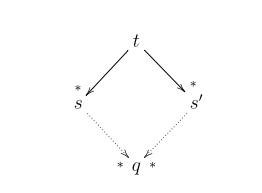
\includegraphics[scale=0.5]{images/konfluenzDiamant.png}
		\item T heißt \textbf{lokal konfluent} (WCR, weakly Church/Rosser) $\iff \forall t,s,s' (t\to s\land t\to s'\implies s,s'\ zf)$ (also in nur einem schritt zusammenführbar)\\
		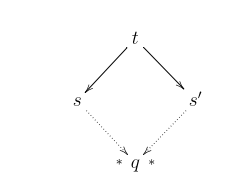
\includegraphics[scale=0.5]{images/WeaklyChurchRosser.png}
	\end{itemize}
	z.B.: ist oben \ref{gruppen} weder stark noch schwach CR
	\end{definition}
	\begin{satz} Sei t konfluent $\implies$\\
	1) $s\leftrightarrow^* t\iff s,t\ zf$\\
	2) $s,s'$ NF von $t\implies s=s'$\\
	\end{satz}
	\begin{beweis}\ \\
	1) $\impliedby$ klar $\implies$\\
	Haben $s=t_0 \leftrightarrow t_1\leftrightarrow \dots\leftrightarrow t_n=t$\\
	Induktion über n:\\
	$n=0: s=t$ klar\\
	$n\to n+1:$ Nach I.V. $s=t_0\to^*q ^*\gets t_n\leftrightarrow t_{n+1}$\\
	Fall 1: $t_n\gets t_{n+1}$ fertig (weil $t_n$ über q mit s zusammenführbar)\\
	Fall 2: $t_n\to t_{n+1}$ dann gibt es ein r, dass über $\to^*$ mit $t_{n+1}$ und $q$ erreichbar ist (wegen konfluenz)\\
	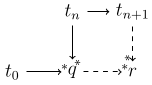
\includegraphics[scale=0.5]{images/symmetrischTransitiverAbschlussKonfluenz.png}\\
	2) $s\leftrightarrow^* s'\implies s,s'\ zf: s\to^* u^*\gets s'$ weil $s,s'$ NF, braucht man genau 0 schritte: $s=u=s'$\\
	\end{beweis}
	hier ein bsp für eine konfluente form:\\
	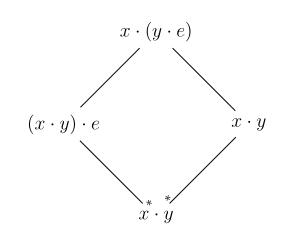
\includegraphics[scale=0.5]{images/konfluent.png}\\
	\begin{satz} (Newman's Lemma)\label{Newman's Lemma}\\
	\[SN \land\ WCR \implies CR\]
	(also lokale konfluenz und stark normalisierend, führt zur vollen konfluenz, starke konfluenz ist i.a untentscheidbar (und so auch SN, deshalb widerspricht dieser Satz dem nicht\dots))
	Beweis, später\\
	\end{satz}
	\begin{beispiel}\ \\
	Regeln\\
	$l_1\to r_1$\\
	$l_2\to r_2$\\
	Terme\\
	$C_1(l_1\sigma_1)=t=C_2(l_2\sigma_2)$\\
	$C_1(l_1\sigma_1)\to C_1(r_1\sigma_1)$\\
	$C_2(l_2\sigma_2)\to C_2(r_2\sigma_2)$\\
	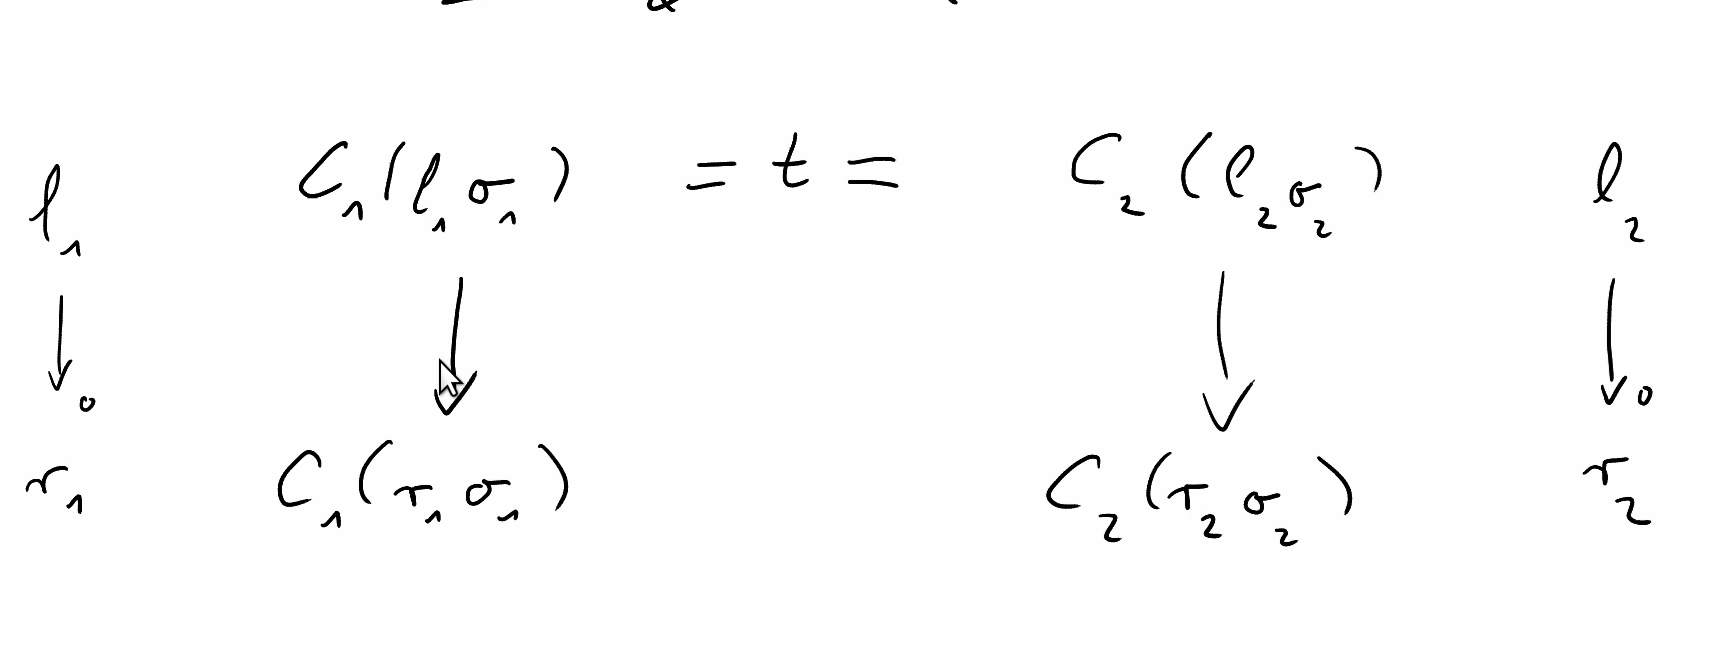
\includegraphics[width=256px]{images/lokaleKonfBspNewmann.png}\\
	$C_1$ kann ignoriert werden wegen kontextabgeschlossen.\\
	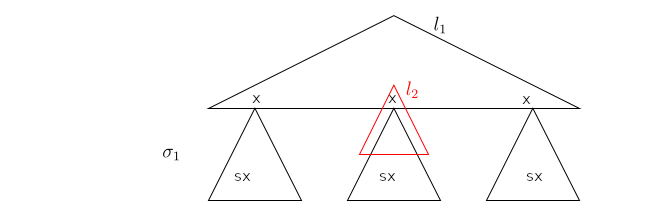
\includegraphics[width=256px]{images/konfluenzbaum.png}\\
	Weil $l_2$ in $l_1$ hineinragt, ist nach anwendung von $l_2\to r_2$ kein $l_1$ mehr für die zweite Regel vorhanden (die eine anwendung zerschiest die prämisse einer zweiten)\\
	\end{beispiel}
	\begin{definition} Unifikation\\
	$t,s$ Terme $t\stackrel{\cdot}{=} s$\\
	$\sigma$ Unifikator von t,s $(\sigma\in Unif(t,s))\iff t\sigma=s\sigma$ (syntaktisch)\\
	$t,s$ unfiz $\iff$ $unif(t,s)\neq \emptyset$\\
	$\sigma$ allgemeiner als $\sigma' \iff\exists \tau ( \sigma' = \sigma\tau)$\\
	$\sigma$ allgemeinster Unifikator (mgu) von $t,s$
	$\sigma = mgu(t,s)\iff \sigma\in Unif(t,s)\land \forall \sigma'\in Unif(t,s)(\sigma \text{allgemeiner als }\sigma')$ mgu existiert, wenn t,s unifizierbar, eindeutig bis auf isomorphismus (injektive umbennennung)\\
	\end{definition}
	\begin{beispiel} unifikation\\
	$k(r(x),x)\stackrel{\cdot}{=} k(z,r(z))$\\
	decomp $r(x)\stackrel{\cdot}{=}z, x\stackrel{\cdot}{=} r(z)$\\
	elim $r(r(z))\stackrel{\cdot}{=}z, x\stackrel{\cdot}{=} r(z)$\\
	occurs.\\
	$f(h(x),z), f(y,g(x))$\\
	$\sigma=[h(x)/y, g(x)/z]$\\
	\end{beispiel}
	\begin{definition}kritisches Paar nach Knuth-Bendix\\
	Seien $l_1\to_0 r_1, l_2\to_0 r_2$,\\
	$l_1 = C(t)$ t nichttrivial (d.h. t keine Variable, konstanten gehen aber\dots)\\
	und $FV(l_2)\cap FV(l_1)=\emptyset$\\
	$\sigma = mgu(t,l_2)$\\
	also, wenn man $r_1\sigma\gets l_1\sigma = C(t)\sigma =( C\sigma(t\sigma) = C\sigma(l_2)\to C\sigma(r_2\sigma)=C(r_2)\sigma$\\
	$\implies (r_1\sigma, C(r_2)\sigma)$  \textbf{kritisches Paar}
	\end{definition}
	\begin{lemma} $(r_1\sigma, C(r_2\sigma))$ kritisches Paar\label{critical pair}\\
	$\implies r_1\sigma\gets l_1\sigma =C(l_2)\sigma \to C(r_2)\sigma$ (kritische Paare sind divergente Redukte eines gemeinsamen ursprungs)
	\end{lemma}
	\begin{korrolar}$T\ WCR\implies$ alle Paare sind zf
	\end{korrolar}
	\begin{satz} alle kritischen Paare zf $\implies WCR$ (Critical Pair Lemma)\label{critical pair lemma}\\
	Aufwand ist $O(n^3)$ (paare und dann jede Regel für kontext C(t) einsetzen, mal die anzahl der Schritte, den jede reduktion selbst benötigt)\\
	\end{satz}
	\begin{beispiel} (Gruppe)\\
	$(l_1\to_0 r_1) = (x\cdot (y\cdot z))\to_0 (x\cdot y)\cdot z)$\\
	(in frische variablen umbennenen)\\
	$(l_2\to_0 r_2) = (x'\cdot e\to x')$\\
	Jetzt: wähle einen Teilterm aus, und mach das ``t'' draus:\\
	$C(\cdot) = x\cdot(\cdot)$\\
	$t=y\cdot z$ $\sigma=mgu(t,l_2) = [y/x',e/z]$\\
	$\to$ kritisches Paar $(r_1\sigma, C(r_2)\sigma) = ((x\cdot y)\cdot e,\ x\cdot y)$\\
	(die $r_1,r_2$ sind oben definiert\dots)\\
	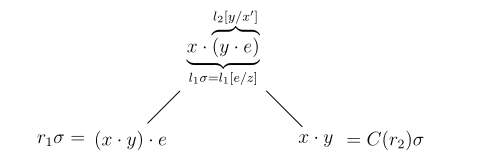
\includegraphics[width=256px]{images/criticalPairs.png}\\
	\end{beispiel}
	\begin{beispiel}\ \\
	$l_1\to_0 r_1 = (x\cdot (y\cdot z))\to_0 (x\cdot y)\cdot z)$\\
	$l_2\to_0 r_2 = (x'\cdot x^{-1'}\to_0 e)$\\
	$C(\cdot) = x\cdot (\cdot)$\\
	$t=y\cdot z$\\
	$\sigma= mgu(t,l_2) = [x'/y, x^{-1'}/z]$\\
	$(x\cdot x')\cdot x^{'-1}\gets x\cdot (x'\cdot x^{-1'})\to x\cdot e$ nicht z.f.\\
	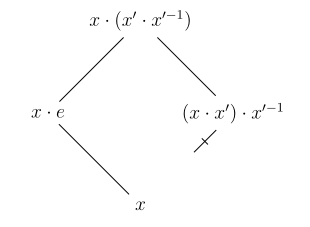
\includegraphics[height=128px]{images/nichtZF.png}\\
	\end{beispiel}
	\begin{beispiel}
	$l_1\to_0 r_1 = (x\cdot(y\cdot z)\to_0 (x\cdot y)z) = l_2\to_0 r_2$\\
	$t=y\cdot z$
	$\sigma = mgu(t,l_2)=mgu((y\cdot z), x'\cdot(y'\cdot z')) = [y/x', y'\cdot z'/z]$\\
	$(x\cdot y) \cdot (y'\cdot z')\gets x\cdot (y\cdot (y'\cdot z'))\to x\cdot ((y\cdot y')\cdot z')$\\
	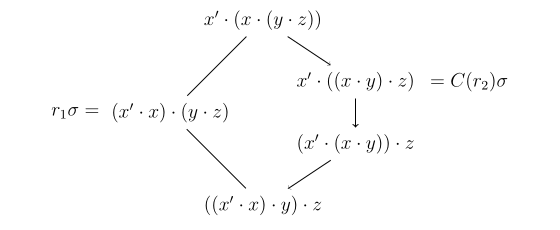
\includegraphics[height=128px]{images/SelbstReferenzCriticalPair.png}\\
	sind z.f.\\
	\textbf{\underline{ACHTUNG}}\\
	wenn man das umbennenen der variablen vergisst, dann krigt man $y\cdot z$ und $x\cdot (y\cdot z)$$\longrightarrow \bot$ occurs!!\\
	\end{beispiel}
	\begin{beweis} Critical Pair Lemma\ref{critical pair lemma}\\
	Notation $C(\cdot) \sqsubseteq D(\cdot)\iff \exists E(\cdot)(C(\cdot)=D(E(\cdot)))$ (also C liegt unter D, wenn man in D einen weiteren kontext einführen kann, um ihn zu C zu verwandeln! Wie bei mgu auch)\\
	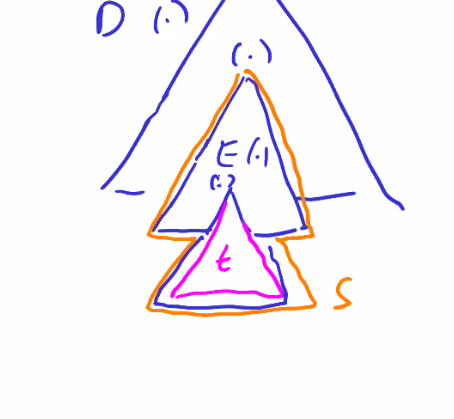
\includegraphics[height=128px]{images/CunterD.png}\\
	$C(\cdot)\bot D(\cdot)\iff C(\cdot)\cancel{\sqsubseteq} D(\cdot)\land D(\cdot)\cancel{\sqsubseteq} C(\cdot)$ (also keiner ist subset des anderen, sie sind orthogonal)\\
	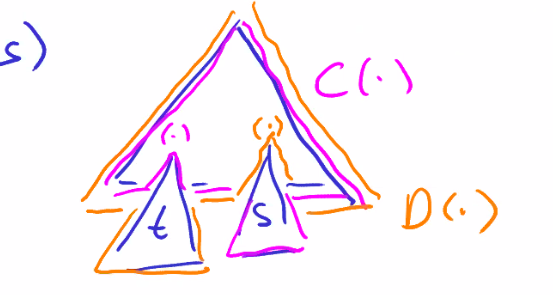
\includegraphics[width=256px]{images/orthogonalKontext.png}\\
	Sei $l_1\to_0 r_1, l_2\to r_2$ anwendbar auf s\\
	\textbf{Fall 1}:$C_1(\cdot)\bot C_2(\cdot)$\\
	\includegraphics[height=128px]{images/unabhängigeKontexte.png}\\
	Beide Terme stören sich nicht, ich kann immer beide Regeln in beliebiger Reihenfolge anwenden\\
	Fall 2: o.b.d.A $C_2(\cdot)\sqsubseteq C_1(\cdot)$ mit $C_1(\cdot) =(\cdot)$ (man kann sich den äußersten einfach wegdenken, der Teilbaum unter einem echten $C_1\neq (\cdot)$ ist equivalent zu einem normalen Baum mit wurzel direkt unter $C_1$)\\
	ohne einschrenkung $l_2\sigma = l_2$, weil $l_2$ sowieso vollkommen unter unserer substitution liegt, also auch im nachhinein gemacht werden kann ( es stört den Rest des Terms nicht).\\
	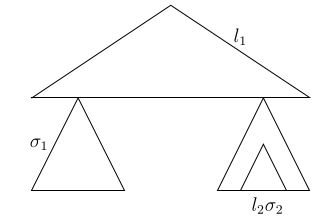
\includegraphics[width=128px]{images/TeilbaumFall.png}\\
	\underline{unterfall 2a)} $C_2$ ist echt unterhalb von $l_1$\\
	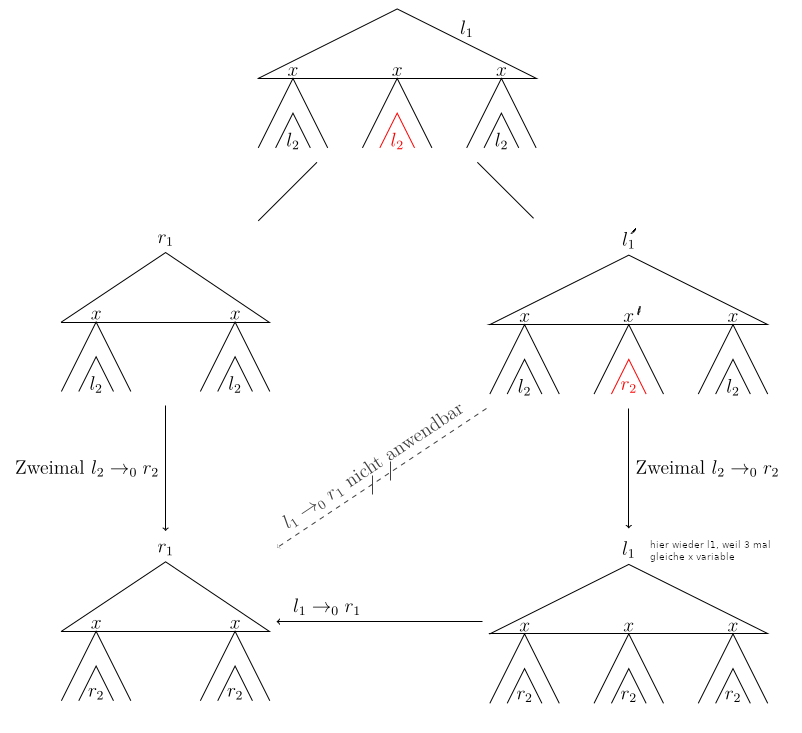
\includegraphics[width=256px]{images/unterfall2a.png}\\
	auf der rechten seite ist $l_1\to r_1$ nicht mehr anwendbar, weil $l_1\to r_1$ fordert, dass es 3 gleiche argumente gibt.\\
	\underline{unterfall 2b)} $C_2$ ist nicht unterhalb von $l_1$, d.h. $(\cdot)$ von $C_2$ liegt in $l_1$:\\
	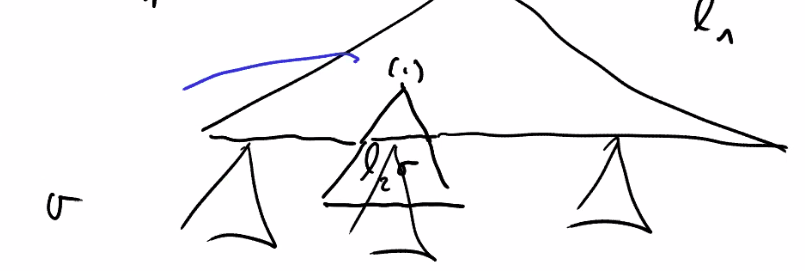
\includegraphics[width=128px]{images/unterfall2b.png}\\
	Dies ist gleich der situation des Kritischen paares \ref{critical pair}: Der einzige ort, wo es schiefgehen kann ist also, wenn das kritische paar nicht zf ist.\\
	Es reicht also: Für $\sigma\in Unif(t,l_2)$ ist $(r_1\sigma, C_2(r_2)\sigma)$ zf.\\
	Gilt nach Annahmen für $\sigma =mgu(t,l_2)$ (alle kritischen paare sind zf), dann $\sigma' =\sigma\tau$ für ein $\tau$\\
	$r_1\sigma\tau, C_2(r_2)\sigma \tau$ unsere Reduktionsrelation ist stabil, also ist $r_1\sigma, C_2(r_2)\sigma$ zf, so auch alle substitutionen.\\
	\end{beweis}
	\begin{satz} wohlfundiert Induktion\\
	$R\subseteq X\times X$ wohlfundiert $\implies$\\
	Wenn $\forall x (\forall y (xRy\implies P(y)))\implies P(x)$ (1)\\
	(wenn für alle nachfolger von x P(y) gilt, dann gilt auch P(x))\\
	dann gilt $\forall x(P(x))$ (2)\\
	dies heißt wohlfundierte Induktion.\\
	\end{satz}
	\begin{beweis} Kontraposition:\\
	zeige $(1)\land \lnot (2)\implies R$ nicht wohlfundiert.\\
	Per $\lnot(2)$ ex. $x_0$ mit $\lnot P(x_0)$\\
	$\stackrel{\implies}{(1)}$ ex. $x_1$ mit $x_0Rx_1$ $\lnot P(x_1)$\dots\\
	d.h. $x_0 Rx_1Rx_2\dots,$ R nicht wf.\\
	\textbf{(dependent choice, viel harmloser als ZFC's auswahlaxiom)}
	\end{beweis}
	\begin{beispiel} 1) $X=\mathbb{N}$ $R=\{(n+1,n)|n\in\mathbb{N}\}$\\
	wohlfundierte Relation (bzw vollständige Relation als wohlfundierte\dots):\\
	$P(0)$\\
	$\forall n(P(n)\implies P(n+1))$\\
	zusammen liefert das $\forall n (P(n))$\\
	\end{beispiel}
	\begin{beispiel} $X=\mathbb{N}$ $R= >:$ Course-of-values-Induktion (man nimmt also für alle echt kleineren n die Aussage an)
	\end{beispiel}
	\begin{beweis} Newman's Lemma \ref{Newman's Lemma} $SN \& WCR\implies CR$\\
	beweis per wohlfundierter Relation über $\to$ (ist wf wegen SN).\\
	o.E. $t\to^+ s,s'$ (weil in 0 schritten reduzieren trivialerweise sofortig zf ist)\\
	Idee: man teilt die schritte zwischen $s$ und $s'$ in jeweils zwei paare von beiden seiten ($s_0, s_0'$) dann Induktionsvorraussetzung anwenden, woraus man folgern kann, dass dies für jeden schritt möglich ist:\\
	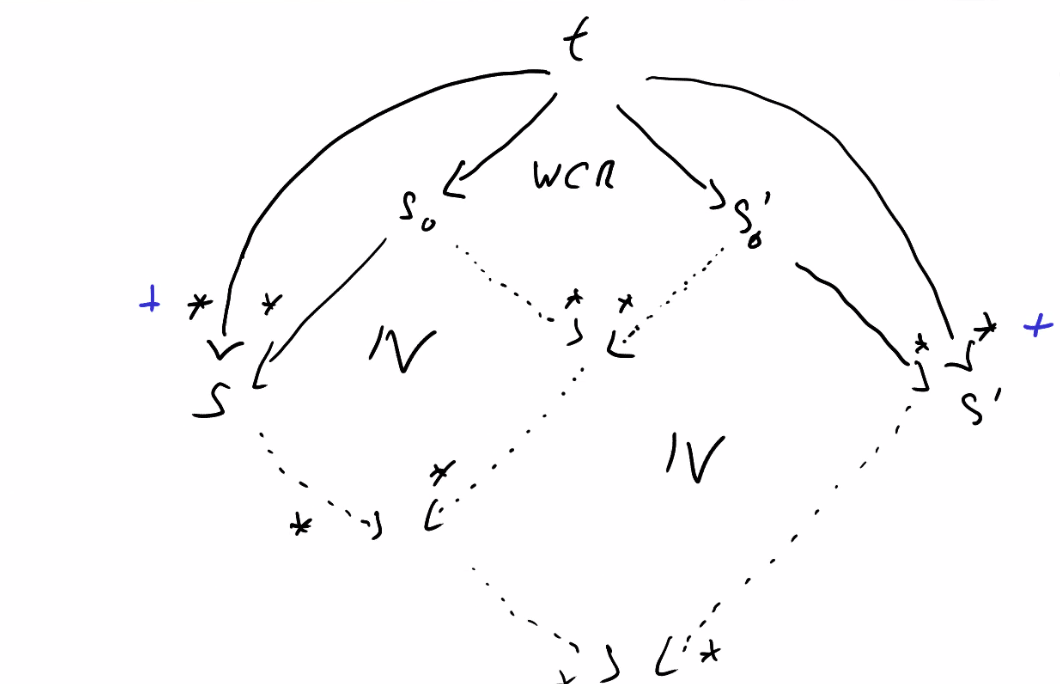
\includegraphics[width=256px]{images/NewmansLemma.png}\\
	\end{beweis}
	\newpage
	\section{Der $\lambda$-Kalkül}
	Beispiel haskell
	\begin{framed}
	\begin{minted}{haskell}
	twice f x = f $ f x
	-- Eigentlich ``Schönfinkelisierung'' nach dem echten Erfinder.
	map:: (a-> b)-> (List a-> List b) 
	map f [] = []
	map f (x:xs) =(f x):map(f xs)
	\end{minted}
	\end{framed}\noindent
	ungetypter $\lambda$-Kalkül = LISP.\\
	getypter $\lambda$-Kalküle\\
	Church (Ein zuerst unvollständiges system), Kleene, Rosser (haben beide R, Curry)\\
	\section{Der ungetypte $\lambda$-Kalkül}
	\begin{definition}
	$\lambda x.t$ ``die Funktion, die x auf t abbildet $x\mapsto t$ (wobei üblicherweise $x\in FV(T)$ ist)''\\
	$ts$ Anwendung von s auf t. (Applikation)\\
	\underline{Terme} t,s gegeben durch:\\
	\[t,s::= x|ts|\lambda x.t\: (x\in V)\]
	Wobei das Zweite als ($\lambda$)-Notation.
	\end{definition}
	\begin{beispiel}\hfill
	\begin{itemize}
	\item ``$\lambda x.3+x$'' (3 und plus ist technisch gesehen nicht definiert\dots)
	\item $\lambda x. xx$ (Haskell würde typfehler liefern, wenn man x als funktion auf sich selbst andwendet, es gibt aber sinnvole kontexte für solche dinge: Wenn x eine berechenbare funktion ist, dann muss es einen bestimmten, Gödelnummerierbaren, funktionsraum geben. Das erste x wäre dann die interpretation als funktion, und die zweite die Gödelnummer)
	\item $\lambda x.\lambda y. x=: f$, dann wäre z.B. $f x y = (\lambda y.x) y = x$
	\end{itemize}
	\end{beispiel}
	\begin{definition} Freie Variablen und konventionen\\
	Kontexte
	 \[C(\cdot)=(\cdot)|tC(\cdot)|C(\cdot)s|\lambda x.C(\cdot)\]
	\textbf{Kongruenz} = Kontextabgeschlossene Äquivalenz.\\
	Notation $\lambda x_1\dots\lambda x_n. t = \lambda x_1\dots x_n.t$\\
	$tsu = (ts)u$\\
	Scope von $\lambda$ so weit wie möglich.\\
	$\lambda x.xx= \lambda x.(xx) $ im gegensatz zu $ (\lambda x.x)x$\\
	Freie Variablen:\\
	$FV(x)=\{x\}$\\
	$FV(ts)=FV(t)\cup FV(s)$\\
	$FV(\lambda x.t)= FV(t)\setminus \{x\}$\\
	\end{definition}
	\begin{definition} Substitution\\
	\begin{itemize}
		\item $x\sigma = \sigma(x)$
		\item $(ts)\sigma = (t\sigma)(s\sigma)$
		\item $(\lambda x.t)\sigma = \lambda y.(t\sigma')$ wobei y eine \textbf{frische variable} ist\\
		(also $y\in FV(\sigma(z)), (z\in FV(t)\setminus\{x\}\iff z\in FV(\lambda x.t))$), sonst könnte x ``gefangen werden'' $\lambda x.y [x/y]\neq \lambda x.x$!! Lösung, wie bei $\forall/\exists$ in GLOIN. (capture-avoiding substitution, liefert hier $\lambda x.y [x/y] = \lambda t.x$, mit $\sigma' =\sigma[x\to t]$) de-Broujin indizes. ($\lambda x.\lambda y. xy= \lambda\lambda. 2\ 1$) oder nominale Mengen\cite{nominaleMengen}
	\end{itemize}
	\end{definition}
	\begin{definition}	$t=_\alpha s$ (sprich ``$\alpha$-äquivalent'')\\
	$\iff $ t geht aus  s durch\textbf{ Umbennenung} gebundener Variablen hervor (ohne Variableneinfang!).\\
	Formal: $=_\alpha$ ist die von
	\[\lambda x.t =_\alpha \lambda y.t[y/x]\: (y\notin FV(t)\setminus\{x\})\]
	erzeugte Kongruenz
	\end{definition}
	\begin{beispiel}\ \\
	$\lambda x.xy =_\alpha \lambda z.zy \cancel{=_\alpha} \lambda y.yy$
	\end{beispiel}
	\begin{lemma} $=_\alpha$ ist stabil
	\end{lemma}
	\begin{beweis} Es reicht: erzeugende Relation ist stabil:\\
	\[R=\{(\lambda x.t, \lambda y.t[y/x])|y\notin FV(\lambda x.t)\}\]
	Sei also $y\notin  FV(\lambda x.t)$\\
	zZ: $(\lambda x.t)\sigma R (\lambda y.t[y/x])\sigma$\\
	Daraus folgt (2) $\lambda x'.t\sigma'$ $\lambda y'.t[y/x]\sigma''$\\
	Wobei $\sigma' = \sigma[x\mapsto x']$ und $\sigma'' = \sigma[y\mapsto y']$ und $x',y'$ frisch\\
	$[y/x]\sigma'' = \sigma'[y'/x']$\\
	$x\to y\to y' = x\to x'\to y'$\\
	somit ist die Rechte seite $\lambda y'.t\sigma [y'/x']$ mit $y'\notin FV(\lambda x'.t\sigma')$ frisch.\\
	Die Rechte seite is talso gleich der linken in (2)\\
	\end{beweis}
	\begin{satz} $\beta$-Reduktion. Operationale Semantik (``Wie sich ein program während der Ausführung verändert'')\\
	Im imperativen gibt es Kontexte:
	$\eta, (x:=1;c)\to \eta[x\mapsto 1];c$ ($\eta$ Umgebung, wie in GLOIN)\\
	In $\lambda$-Kalkül gibt es sowas nicht: $\beta$-Reduktion als kontextabgeschlossene Umformung\\
	$(\lambda x.3+x)3\to 3+4(\to \text{ wenn + bekannt ist})$\\
	$\lambda-$Kalkül ist im wesentlichen ein TES (nicht 100\% wegen alpha-equiv und gebundenen Variablen)\\
	$(\beta) \ (\lambda x.t)x\to_0 t$\\
	$\implies$ Einschrittreduktion $\to$\\
	$C((\lambda x.t)s)\to C(t[s/x])$\\
	$(\lambda x.t)s$ heißt $\beta$-Redex.[hier nicht: $(\eta)\ \lambda x.y x\to_0 y$, beliebt in theoriebetrachtung, aber nicht in programmiersprachen (wenn man Seiteneffekte/IO hat, macht $(\eta)$ viel kaputt, weil damit die ``ausführung'' von x auf y umgangen wird)]\\
	\end{satz}
	\begin{beispiel}\ \\
	\begin{itemize}
		\item $(\lambda x.xx)(y x)\to_\beta y x(y x)$
		\item $(\lambda xy.x(yx))zu\to_\beta \lambda y.z(yz)u\to_\beta z(uz)$
		\item $\omega:=\lambda x.xx$, $\omega\omega= (\lambda x.xx)\omega \to_\beta = \omega\omega\to_\beta\dots$ Nicht terminierend.
		\item Booleans ``$x\times x \to x$''\\
		 $true:=\lambda xy.x$ $false:=\lambda xy.y$\\
		\item Paare: ``$Paar \equiv Fkt$'' $Bool\to x$\\
		 \begin{itemize}
		 	\item $fst:= \lambda p.p true$
		 	\item $snd : = \lambda p.p false$
		 	\item $pair:= \lambda xy.\lambda z.zxy$ wobei ``z eine von true/false ist''
		 \end{itemize}
		 Dies liefert uns:\\
		 $\underline{fst\ \underline{(pair\ x\ y)}}\to_\beta fst (\lambda xy.\lambda zxy)xy\to_{2\times\beta} fst(\lambda z.zxy)=(\lambda p.p\ true)\lambda z.zxy\to_\beta (\lambda z.zxy)true\to_\beta true\ xy=(\lambda xy. x)xy \to_\beta (\lambda y.x)y\to_\beta x$\\
	\end{itemize}
	\end{beispiel}
	\subsection{Rekursion}
	$fact =\lambda n. \text{if n=0 then 1 else n*fact(n-1)}$\\
	Dieser Aufruf besteht aus einer primitiven rekursionsfunktion F und der funktion selbst.$fact = F\ fact$\\
	$F=\lambda f.\lambda n. \text{if n=0 then 1 else n*f(n-1)}$ F nennt man auch ein Funktional.\\
	$fact = F\ fact$ nennt man Fixpunktgleichung. (rekursive Funktionen sind Fixpunktgleichen)\\
	Fixpunktkombinator fix:\\
	fix F = F(fix F)\\
	\begin{satz} $\lambda$-Kalkül Fixpunktkombinator\\
	1) Jedes t hat einen Fixpunkt s, d.h. $s\to_\beta ts$ (also die Reduktion liefert wieder ts auf dem wider reduziert werden kann, ad absurdum)\\
	2) Es existiert ein Fixpunktkombinator Y, d.h. $Yt\to_\beta s$ s ist Fixpunkt von t\\
	$Yt\to_\beta s\stackrel{(1)}{\to_\beta} ts$\\
	\end{satz}
	\begin{beweis} \ \\
	1) $s=W_tW_t, W_t = \lambda x.t(xx)$ (wie oben bei $\omega\omega$, bloß mit t ausenrum):\\
	$s=W_tW_t =(\lambda x.t(xx))W_t\to_\beta t(W_tW_t) = ts$\\
	2) $Y=\lambda f.W_fW_f$ wenn man das jetzt auf ein f anwendet erhält man genau $fs=s$
	\end{beweis}
	\begin{beispiel}
	Der Fall von oben $\lambda x.xx =\omega$ und dann $\omega\omega$ hat die funktion $t=\omega$ terminiert deshalb nicht.\\
	$\lambda x.((\lambda y.y)(xx))$ jetzt $t=\lambda y.y$ (also rekursion über die Identitätsfunktion) und s wäre dann $\omega\omega\to_\beta t(\omega\omega)\to_\beta \omega\omega$
	\end{beispiel}
	\subsection{Auswertungsstrategie}
	\begin{beispiel}\ \\
	$(\lambda xy.x)x(\omega\omega)$ Wenn man probiert zuerst $\omega\omega$ zu reduzieren, läuft man undendlich weiter.\\
	Wenn man den rechten reduziert erhält man:\\
	$(\lambda y.x)(\omega\omega)$ wo man entweder wieder ad absurdum $(\omega\omega)$ reduzieren kann (ML, leftmost-innermost, applikativ), oder das ganze zerlegen in:\\
	$\lambda y.x \omega \omega = x$ (Haskell, leftmost-outermost, normal/standard)\\
	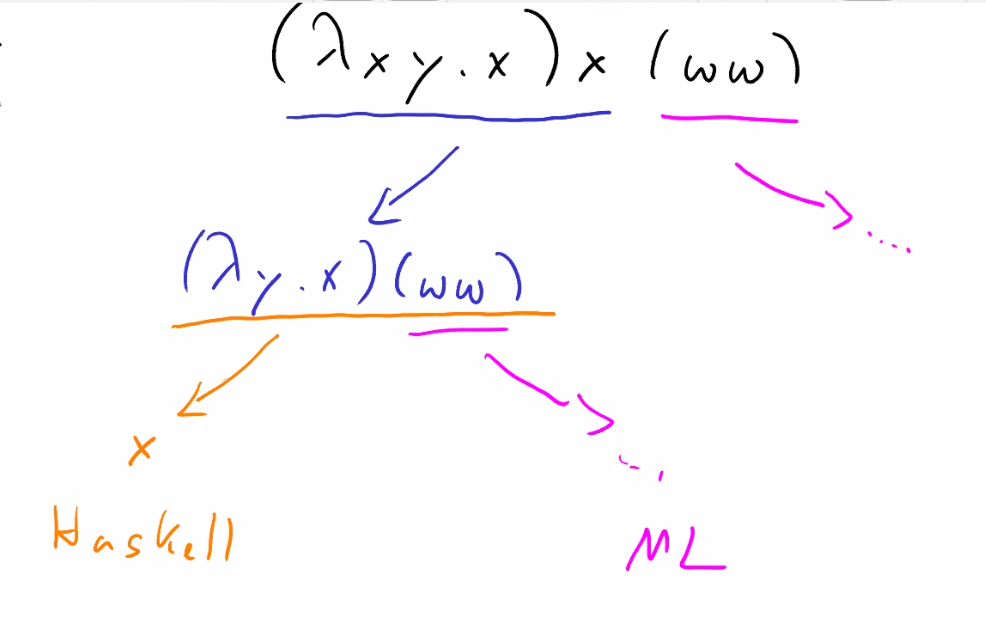
\includegraphics[width=256px]{images/AuswertungsReihenfolge.png}
	\end{beispiel}
	\begin{definition} applikative (leftmost-innermost) Reduktion $\to_a$\\
	induktiv definiert durch:\\
	1a)$(\lambda x.t)s\to_a t[s/x]$ \textbf{wenn} t,s normal (innermost, eager).\\
	2a) $(\lambda x.t\to_a \lambda x.t')$, wenn $t\to_a t'$ (eine echte prog. sprache macht aber niemals Termreduktionen unter einem lambda)\\
	3a)$ts\to_a t's$ wenn $t\to_a t'$\\
	4a)$ts\to_a ts'$, wenn $s\to_a s'$ und t normal.
	\end{definition}
	\begin{definition} normale (leftmost-outermost) Reduktion $\to_n$\\
	1n) $(\lambda x.t)s\to_n t[s/x]$ immer (outermost reinziehen)\\
	2n) $\lambda x.t\to_n \lambda x.t'$, wenn $t\to_n t'$\\
	3n) $ts\to_n t's$, wenn $t\to_n t'$ und t keine $\lambda-$Abstraktion. (wenn es eine wäre, dann 1. Regel)\\
	4n) $ts\to_n ts'$ wenn $s\to_n s'$ und t normal und keine $\lambda$-Abstraktion.\\
	\end{definition}
	\begin{beispiel} $(\lambda y.x)(\omega\omega)$\\
	mit normaler Reduktion:\\
	$(\lambda y.x)(\omega\omega)\to_{1n} x$\\
	mit Applikativer Reduktion:\\
	$(\lambda y.x)(\omega\omega)\to_{4.a} (\lambda y.x)(\omega\omega)$
	\end{beispiel}
	\begin{satz} Standardisierungssatz:\\
	Sei $t\to^* s$ s Normalform $\implies t\to_n^* s$\\
	(Nebenbemerkung: $(\lambda x.fxx)t\to_n ftt\to_n fst\to_nfss$ und $(\lambda x.fxx)t\to_a (\lambda x.fxx)s\to_a fss$ also geht es mit applikativen schneller, weil man funktionen nur 1 mal evaluieren muss)
	\end{satz}
	\section{Der einfach getypte $\lambda$-Kalkül}
	Typen $\alpha,\beta$:\\
	$\alpha\to\beta$ Funktion von $\alpha$ nach $\beta$\\
	Typvariablen a,b,\dots\\
	z.B. $\lambda x.x:a\to a$\\
	\begin{definition}\ \\
	Gegebene Menge $\bold{V}$ var.\\
	Typvariablen $\bold{B}$ von Basistypen.\\
	($\bold{bool,Int,\dots}$) sind typen $\alpha,\beta,\dots$\\
	definiert durch
	\[\alpha,\beta::= a|\bold{b}|\alpha\to\beta\ (a\in\bold{V},\bold{b}\in\bold{B})\]
	z.B. $a\to(b\to a) = (a\to b)\to a = a\to b\to a$
	Terme: Church: $\lambda x:\alpha.t$ nur typkorrekte Terme. (also termbildung und typisierung)\\
	Curry: $\lambda x.t,$ Term kann typisierbar sein oder nicht.\\
	$\omega =\lambda x.xx$ z.B. nicht typisierbar ($\lambda \to$, weil typ voll rekursiv ist)\\
	wir benützen curry.
	\end{definition}
	$x\lambda y.y$ ? weil x unbekannt/untypisiert.\\
	\begin{definition} kontexte\label{typkontext}\\
	Ein Kontext ist eine endliche Menge $\Gamma$ von Typisierungsannahmen $x:\alpha (x\in V)$ ``x hat typ $\alpha$''\\
	Schreibweise: $\Gamma, x:\alpha = \Gamma \cup \{x:\alpha\}$\\
	d.h. $\Gamma$ ist eine endliche partielle Abbildung. (von variablennamen auf typen)\\
	Typisierungsurteile (typing judgements) $\Gamma \vdash t:\alpha $ ``in Kontext $\Gamma$ hat t Typ $\alpha$''
	z.B. $f:a\to b, x:a\vdash fx:b$\\
	Herleitbarkeit induktiv:\\
	\AxiomC{}
	\RightLabel{$ (x:\alpha)\in\Gamma$}\\
	\LeftLabel{(Ax)}
	\UnaryInfC{$\Gamma \vdash x:\alpha$}
	\DisplayProof\\
	\AxiomC{$\Gamma\vdash t:\alpha\to \beta$}
	\AxiomC{$\Gamma \vdash s:\alpha$}
	\LeftLabel{($\to_e$)}
	\BinaryInfC{$\Gamma \vdash ts:\beta$}
	\DisplayProof\\
	\AxiomC{$\Gamma[x\mapsto \alpha]\vdash t:\beta$}
	\LeftLabel{($\to_i$)}
	\RightLabel{(also wenn x schon einen typ hat, wird dieser Überschrieben, shadowing)}
	\UnaryInfC{$\Gamma \vdash\lambda x.t:\alpha\to\beta$}
	\DisplayProof\\
	Rechts: sonst könnte $x:\alpha$ zum clash führen! ( in der Realität könnte man das lösen, indem man aus $\Gamma$ eine List statt eine Menge baut)\\
	\end{definition}
	\begin{beispiel}\ \\
	\\
	\LeftLabel{$Ax$}\AxiomC{}\AxiomC{}\RightLabel{$AX$}
	\BinaryInfC{$\vdash x: a\to b, y: a\vdash x:a\to b, x: a\to b, y:a \vdash y:a$}
	\UnaryInfC{$\vdash x:a\to b, y:a \vdash xy:b $}
	\LeftLabel{$\to_i$}
	\UnaryInfC{$\vdash x: a\to b\vdash \lambda y.xy: a\to b$}
	\LeftLabel{$\to_i$}
	\UnaryInfC{$\vdash\lambda xy.xy: (a\to b)\to(a\to b)$}
	\DisplayProof\\

	\RightLabel{CIRCULAR DEPENDENCY}
	\AxiomC{$x:a \to \vdash x:a \to x:a\to \vdash x:a$}
	\LeftLabel{$\to_e$}
	\UnaryInfC{$x: \vdash xx$}
	\LeftLabel{$\to_i$}
	\UnaryInfC{$\vdash\lambda x.xx: $}
	\DisplayProof\\
	\end{beispiel}
	Berechnungsprobleme:\\
	\begin{itemize}
		\item gilt $\vdash t:\alpha$ ? (typcheck)
		\item finde (existiert?) $\alpha$ mit $\vdash t:\alpha$ (Typinferenz)
		\item finde (existiert?) t mit $\vdash t:\alpha$ (Type inhabitation)
	\end{itemize}
	\begin{beispiel}
	$a\to a$ inhabited (Identitätsfunktion $\lambda x.x$, bildet typ auf sich selbst ab, nach curry-howard tautologie)\\
	$a$ nicht inhabited (also für sich stehend hat ein wert nicht irgendeinen typ, nicht obdA gültig)\\
	$(a\to a)\to a$ nicht inhabited (das erste ist eine Tautologie, also immer wahr, a selbst ist aber nicht immer wahr)\\
	denn: wäre $\vdash t: (a\to a)\to a$, dann $t(\lambda x.x):a$ widerspruch! (dependent Types a'la idris/agda, Programmsynthese, automatisches Beweisen)
	\end{beispiel}
	Eigenschaften:\\
	\AxiomC{$\phi(c)$}
	\RightLabel{$\forall I$}
	\LeftLabel{c frisch}
	\UnaryInfC{$\forall (\phi)$}
	\DisplayProof\\
	\AxiomC{$\phi\vdash \psi$}
	\RightLabel{$\to I$}
	\UnaryInfC{$\phi\to \psi$}
	\DisplayProof\\

	\AxiomC{$\phi(c)\vdash \psi(c$)}
	\RightLabel{herleitbar:}
	\LeftLabel{c frisch}
	\UnaryInfC{$\forall x(\phi\to \psi)$}
	\DisplayProof\\
	Beweis:\\
	\AxiomC{$\phi\vdash \psi$}
	\UnaryInfC{$\phi(c)\to \psi(c)$}
	\RightLabel{c frisch}
	\LeftLabel{$\forall I$}
	\UnaryInfC{$\forall x(\phi\to \psi)$}
	\DisplayProof\\
	Regel zulässig $\iff$ durch ihre Hinzunahme wird nichts neu herleitbar.\\
	\begin{lemma} (Weakening)\\
	\AxiomC{$\Gamma \vdash t:\alpha$}
	\RightLabel{$\Gamma\subseteq \Gamma'$}
	\LeftLabel{(wk)}
	\UnaryInfC{$\Gamma' \vdash t:\alpha$}
	\DisplayProof\\
	(also ein größerer Kontext ändert nichts an der Herleitbarkeit)
	\end{lemma}
	\begin{beweis} Induktion über Herleitung von $\Gamma\vdash t:\alpha$\\
	$(Ax) \Gamma \vdash x:\alpha, x:\alpha \in \Gamma \implies x:\alpha\in \Gamma'\implies \Gamma'\vdash x:\alpha$
	\AxiomC{$\Gamma[x\mapsto \alpha]\vdash t:\beta$}
	\LeftLabel{($\to_i$)}
	\UnaryInfC{$\Gamma\vdash \lambda x.t:\alpha\to\beta$}
	\DisplayProof\\
	(*) Nach IV. (prämisse ist kleineres Gamma als konklusion) $\Gamma'[x\mapsto \alpha]\vdash t:\beta$\\
	da $\Gamma[x\mapsto \alpha]\subseteq \Gamma'[x\mapsto \alpha]$\\
	Sei $y:\beta\in \Gamma[x\mapsto \alpha]$ (also ein beta ist links, so muss es auch rechts sein)\\
	Fall 1: $y\neq x\implies y:\beta\in \Gamma \implies y:\beta\in \Gamma'\implies y:\beta\in \Gamma'[x\mapsto \alpha]$\\
	Fall 2: $y=x\implies \beta=\alpha \implies y:\beta =x:\alpha\in\Gamma[x\mapsto \alpha]$\\
	per (*) $\to_i$ $\Gamma'\vdash \lambda x.t:\alpha\to\beta$ (die prämisse gilt, also kann man auch die gleiche folgerung machen)
	\end{beweis}
	\begin{lemma} Inversion\\
	(man kann alle Regeln auch umdrehen)\\
	\begin{itemize}
	\item 1) $\Gamma\vdash x:\alpha\implies (x:\alpha)\in\Gamma$ (ax inversion)\\
	\item 2) $\Gamma\vdash ts:\beta \implies$ es existiert $\alpha$ mit $\Gamma\vdash t:\alpha\to\beta$ ($\to_e$ inversion, also wenn es eine Anwendung gibt, dann muss es eine Funktion dazu gegeben haben)\\
	\item 3) $\Gamma\vdash \lambda x.t:\gamma\implies \gamma$ hat die Form $\alpha\to\beta$ und $\Gamma[x\mapsto \alpha]\vdash t:\beta$ ($\to_i$ inversion, also der type des input einer Funktion muss herleitbar sein)
	\end{itemize}
	\end{lemma}
	\begin{beweis} Regeln sind syntaxgerichtet\end{beweis}
	\subsection{Typinferenz}
	$\lambda x.x:a \to a$\\
	$\lambda x.x:(a\to b)\to(a\to b)$\\
	Offensichtlich ist das erst besser als das zweite. Es muss also eine ``Algemeinheitshierarchie'' geben (most general typing)\\
	\begin{definition}
	Terminologie/Notation:\\
	$TV(\alpha)=$ Menge der in $\alpha$ vorkomenden Typvariablen.\\
	$TV(\Gamma)=\bigcup\limits_{(x:\alpha)\in\Gamma}TV(\alpha)$\\
	\underline{Typsubstitution} = Substitution von Typen für  Typvariablen
	$\sigma$ \underline{Lösung} von $\Gamma\vdash t:\alpha$, wenn $\Gamma\sigma\vdash t:\alpha\sigma$ herleitbar.\\
	allgemeinste Lösung (wie bei mgu $\sigma' =\sigma \theta$ dann ist $\sigma$ das allgemeinere, wenn das $\forall \sigma'$ gilt dann ist $\sigma$ die allgemeinste Lösung)\\
	\underline{Prinzipaltyp} von $\Gamma\vdash t=$ allgemeinste Lösung von $\Gamma\vdash t:a$ a frisch $(a\notin TV(\Gamma))$ (prinizipaltyp ist allgemeinste Lösung mit frischen typen und eindeutig modulo Umbennenung)\\
	$\Gamma\vdash t$ \underline{typisierbar} $\iff$ $\Gamma\vdash t:a$ hat eine Lösung. (a frisch)\\
	\end{definition}
	\begin{satz} Algorithmus W nach HINDLEY/MILNER\\
	Berechne zu $\Gamma\vdash t:\alpha$ (``Ziel'')\\
	$PT(\Gamma; t;\alpha)$ Menge von Typgleichungen $a\doteq \beta$ mit $PT(\Gamma;t;\alpha)$ unfizierbar $\iff \Gamma\vdash t:\alpha$ hat Lösung.\\
	$mgu(PT(\Gamma;t;\alpha))$ liefert allgemeinste Lösung von $\Gamma\vdash t:\alpha$ (liefert und ist nicht gleich, weil der PT mehr variablen substituiert als notwendig)\\
	$\implies mgu(PT(();t;a))(a) = $ Prinzipaltyp von t (a frisch, t geschlossen)\\
	Implizit geht man bei diesen Regeln immer von $x\in\Gamma$ aus
	\begin{itemize}
		\item $PT(\Gamma; x;\alpha) =\{\alpha\doteq \beta|x:\beta\in\Gamma\}$ (nach Ax inversionslemma)
		\item $PT(\Gamma; ts;\alpha) =PT(\Gamma;t;a\to \alpha)\cup PT(\Gamma;s;a)\ \textbf{global} (a\ frisch) $ nach $(\to_e)$
		\item $PT(\Gamma; \lambda x.t;\alpha) = PT(\Gamma[x\mapsto a];t,b )\cup \{a\to b\doteq\alpha\}$ mit a,b \textbf{global} frisch $(\to_i)$ invers. (wir fitten also input auf a und output auf b)
	\end{itemize}
	Das global ist notwendig, um einfang bei unifikation zu vermeiden. Lösung z.b. über \cite{nominaleMengen}
	\end{satz}
	\begin{beispiel}\ \\
	$\vdash \lambda xy.xy$\\
	$PT(\emptyset,\lambda xy.xy;a)= PT(x:b,\lambda y.xy,c)\cup \{a\doteq b\to c\} =\\
	PT(x:b,y:d; xy;e)\cup \{a\doteq b\to c,c\doteq d\to e\}\\
	PT(x:b,y:d; x;f\to e)\cup PT(x:b,y:d;y;y:f)\cup \{a\doteq b\to c,c\doteq d\to e\}\\
	= \{b\doteq f\to e, y\doteq f, a\doteq b\to c, c\doteq c=d\to e\}$\\
	jetzt hat man gleichungen, die man unifizieren muss:\\ 
	$mgu = [f/d,f\to e/c,f\to e/b, (f\to e)\to(f\to e)/a]$ wir haben oben mit a angefangen, also ist der endtyp $\lambda xy.xy: (f\to e)\to(f\to e)$ ist Prinzipaltyp.\\
	\\
	$PT(x:a; x\lambda z.z; c) = PT(x:a; x; b\to c)\cup PT(x:a, \lambda z.z; b) = \{a\doteq b\to c\}\cup PT(x:a, z:d; z;e)\cup\{b\doteq d\to e\} = \{a\doteq b\to c, d\doteq e, b\doteq d\to e\}$\\
	$mgu = [e\to e/b, e\to e\to c/a, c/c]$ ``$e\to e\to c/a, c/c$'' also ist Prinzipaltyp.\\
	\\
	$PT(\emptyset; \lambda x.xx, a) = PT(x:b; xx; c )\cup \{a\doteq b\to c\} = PT(x:b; x;d\to c)\cup PT(x:b; x; d) \cup \{a\doteq b\to c\} = \{b\doteq d\to c, b\doteq d,\dots\}$\\
	Unifikation liefert occurs $\bot$ nach substitution [d/b]
	\end{beispiel}
	\begin{satz} $(\Gamma,t)$ typisierbar $\iff$ $PT(\Gamma;t; a)$ (a frisch) unifizierbar; dann $mgu(PT(\Gamma;t; \alpha))|_{TV(\Gamma)\cup \{a\}}$ Prinzipaltyp von $(\Gamma;t)$
	\end{satz}
	\begin{beweis} Zeige allgemeiner:
	\[PT(\Gamma; t;\alpha)\; \text{unifizierbar}\iff \Gamma \vdash t:\alpha\; \text{lösbar}\]
	dann
	\[mgu(PT(\Gamma;t;\alpha))|_{TV(\Gamma,\alpha)} \]
	allgemeinste Lösung von $\Gamma\vdash t:\alpha$\\
	Zeige dazu:\\
	\[\Gamma\sigma\vdash t:\alpha\sigma\iff \sigma\text{ ist erweiterbar zu }\sigma'\in Unif(PT(\Gamma; t; \alpha))\]
	d.h. $\sigma'|_{TV(\Gamma,\alpha} = \sigma$ sigma ist also erweiterbar.\\
	per Induktion über t:\\
	``$\impliedby$'': per Typregeln(\ref{typkontext}).\\
	z.B. $t=\lambda x.s:$\\
	haben $\sigma'\in Unif(PT(\Gamma[x\mapsto a]; s; b)\cup \{\alpha \doteq a\to b\})$\\
	Nach IV. $\underbrace{\Gamma[x\mapsto a]\sigma'}_{=\Gamma[x\mapsto a]\sigma}\vdash s:\underbrace{b\sigma'}_{b\sigma}$\\
	Per ($\to_e$)
	\AxiomC{$\Gamma[x\mapsto a]\sigma$}
	\AxiomC{$s:b\sigma$}
	\BinaryInfC{$\Gamma\sigma\vdash \lambda x.s:a\sigma'\to b\sigma'$}
	\DisplayProof\\
	Daraus folgt $\alpha\sigma'=\alpha\sigma$\\
	\\
	``$\implies$'' Per Inversion:\\
	1.$\Gamma\sigma\vdash x:\alpha\sigma\stackrel{inversion}{\implies}x:\beta\in\Gamma, \alpha\sigma=\beta\sigma$\\
	$\implies \sigma\in Unif(\underbrace{PT(\Gamma;x;\alpha)}_{\alpha\doteq\beta})$\\
	2. $\Gamma \sigma \vdash ts:\alpha\sigma\stackrel{Inversion}{\implies}$\\
	es existiert ein $\gamma$ mit $\Gamma\sigma\vdash t:\gamma\to \alpha\sigma,\Gamma\sigma\vdash s:\gamma$\\
	Setze $\sigma'=\sigma[a\mapsto \gamma]$ (a 	global frisch) $\implies \Gamma\sigma'\vdash t:(a\to \alpha)\sigma',\Gamma\sigma' \vdash s:a\sigma'$\\
	$\stackrel{IV}{\implies} \sigma'$ erweitert zu $\underbrace{\sigma''\in Unif(PT(\Gamma;t;a\to \alpha))}_{\text{gemeinsame TV sind nur die aus} TV(\Gamma;\alpha;a)}$ und $\sigma''\in Unif(PT(\Gamma;s;a))$\\
	$\implies$ $\sigma''\in Unif(PT(\Gamma,ts,\alpha))$\\
	3. $\Gamma\sigma\vdash\lambda x.s:\alpha\sigma\stackrel{Inversion}{\implies}$\\
	$\alpha\sigma = \beta\to\gamma$ $\Gamma\sigma[x\mapsto \beta]\vdash s:\gamma$\\
	Setze $\sigma' =\sigma[a\mapsto \beta,b\mapsto \gamma]$, a,b global frisch\\
	$\implies$ $\Gamma[x\mapsto a]\sigma'\vdash s:b\sigma'$\\
	$\stackrel{IV}{\implies}\sigma'$ erweitert zu $\sigma''\in Unif(PT(\Gamma[x\mapsto a];s; b))$\\
	$\stackrel{(a\to b)\sigma'' = \alpha\sigma''}{\implies} \sigma'' \in Unif(PT(\Gamma; \lambda x.s;\alpha))$\\
	(Das letzte folgt daraus, dass $\alpha\sigma= \beta\to \gamma$ ist und wir $\sigma' =\sigma[a\mapsto \beta,b\mapsto \gamma]$ haben)
	\end{beweis}
	\subsection{Subjektreduktion}
	\begin{satz} $\Gamma\vdash t:\alpha, t\to_\beta s\implies \Gamma \vdash s:\alpha$\\
	\danger{} ``$\impliedby$'' gilt \textbf{NICHT}: z.B. $t=(\lambda x.y)(\lambda x.xx)\to_\beta y$
	\end{satz}
	\begin{lemma} Substitution\\
	$\Gamma[x\mapsto \alpha]\vdash t:\beta, \Gamma\vdash s:\alpha\implies \Gamma\vdash t[s/x]:\beta$\\
	Beweis: induktion über t.
	\end{lemma}
	\begin{beweis} $t= C((\lambda x.u)v), s= C(v[u/x])$\\
	Induktion über $C(\cdot)$\\
	z.B.: $C(\cdot) =(\cdot)$ Per inversion:\\
	$\Gamma\vdash \lambda x.u:\beta\to\alpha, \Gamma\vdash v:\beta$\\
	$\Gamma[x\mapsto\beta]\vdash u:\alpha$\\
	$\stackrel{subst-lemma}{\implies} \Gamma\vdash \underbrace{u[v/x]}_{s}:\alpha$
	\end{beweis}
	\section{Church Rosser des $\lambda$-Kalkül}
	(Dies ist der Ursprüngliche Church-Rosser beweis, der Name wird jetzt mittlerweile für alle TES benutzt).\\
	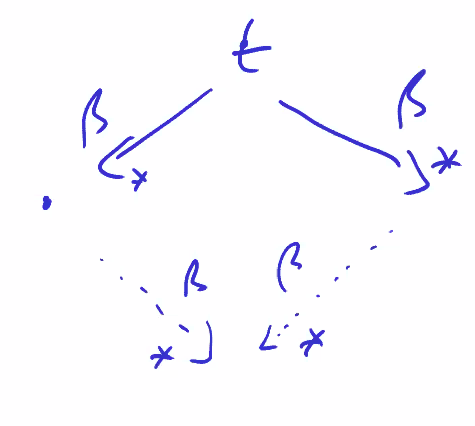
\includegraphics[width=256px]{images/KonfluenzLambda.png}\\
	\begin{lemma} Streifenlemma (strip-lemma)\\
	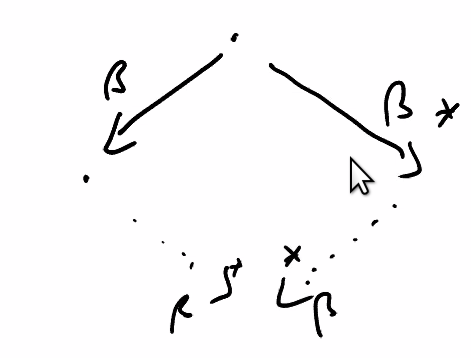
\includegraphics[width=256px]{images/streifenlemma.png}\\
	Effektiv ein mittelweg zwischen WCR und CR.
	\end{lemma}
	Daraus folgt CR:\\
	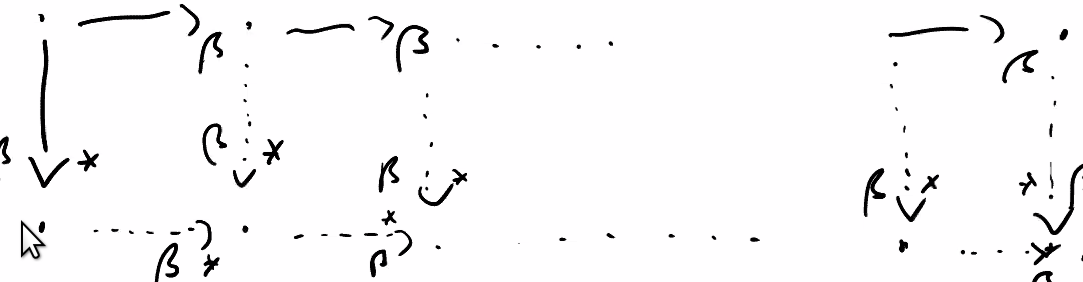
\includegraphics[width=256px]{images/StreifenGenau.png}\\
	oben hat man die n-beta-reduktionen. Unten macht man jeweils immer einen Schritt und kaskadiert nach links.\\
	Dies geht für jedes TES.\\
	Speziell für lambda sähe das so aus.\\
	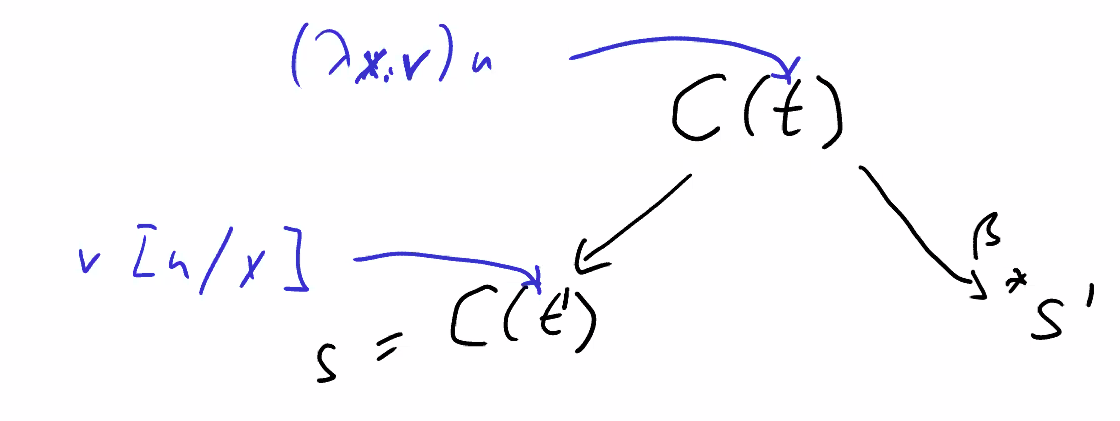
\includegraphics[width=256px]{images/lambdaStreifenlemma.png}\\
	markierte Terme: $t,s::=x|ts|\lambda x.t|(\underline{\lambda}x.t)s$ (also genau gleich, man kann nur \textbf{beta-reduzierbare }terme markieren).\\
	Diese unterstriche müssen wieder ``unlocked'' werden.\\
	$|t|:$ Entfernt \_ aus t, z.B. $|(\underline{\lambda}x.t)s|=(\lambda x.|t|) |s|$\\
	$\phi(t)$ Reduziere alle unterstrichenen Redexe:
	\begin{itemize}
	\item $\phi(x)=x$
	\item $\phi(ts)=\phi(t)\phi(s)$
	\item $\phi(\lambda x.t)=\lambda x.\phi(t)$
	\item $\phi((\underline{\lambda }x.t)s) = \phi(t)[\phi(s)/x]$
	\end{itemize}
	\newcommand{\tomark}{\stackrel{|\cdot|}{\to}}
	Syntaktic sugar $t\tomark |t|$
	\begin{lemma} Lemma A\\
	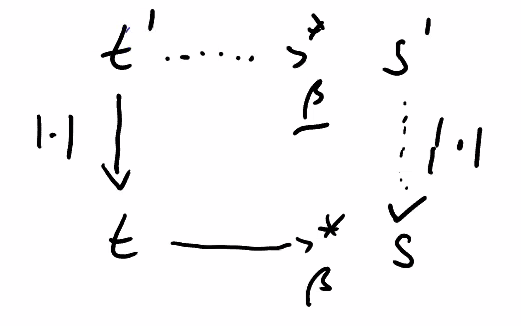
\includegraphics[width=256px]{images/LemmaA.png}\\
	Dabei $(\lambda x.t)s\to_{\underline{\beta}} t[s/x]$ $(\underline{\lambda} x.t)s\to_{\underline{\beta}} t[s/x]$ Es ignoriert also die Unterstriche.\\
	\end{lemma}
	\begin{beweis} Reduziere auf $t\to_\beta s$, Induktion über Kontexte
	\end{beweis}
	Wir bekommen also nicht mehr dazu, oder verlieren ausdruckskraft.
	\begin{lemma} Syntaktisches Substitutionslemma\\
	\[u[v/y][s/x] = u[s/x][v[s/x]/y]\]
	nicht simultan! Das v wird vom x beeinflusst.\\
	wenn $y\notin FV(s), x\neq y$ (bei dem ersten hätte man eine doppelsubstitution, beim zweiten wird die zweite reduktion void)\\
	\end{lemma}
	\begin{beweis} Induktion über u (weil in diesen Reinsubstituiert wird)\\
	Der interessante Fall ist hier der Induktionsanfang, weil im I.S nur weitergereicht wird.\\
	Sei n eine Variable. (LHS/RHS =Left/Right handed side)\\
	$u\notin \{x,y\}\checkmark$\\
	$u= x: LHS = s, RHS=s\text{ weil }y\notin FV(s)$\\
	$u= y:LHS = v[s/x], RHS=v[s/x]$\\
	\end{beweis}

	\begin{lemma} Lemma B\\
	a) $\phi(t[s/x])=\phi(t)[\phi(s)/x]$\\
	b) $\phi$ bewahrt $\beta$\\
	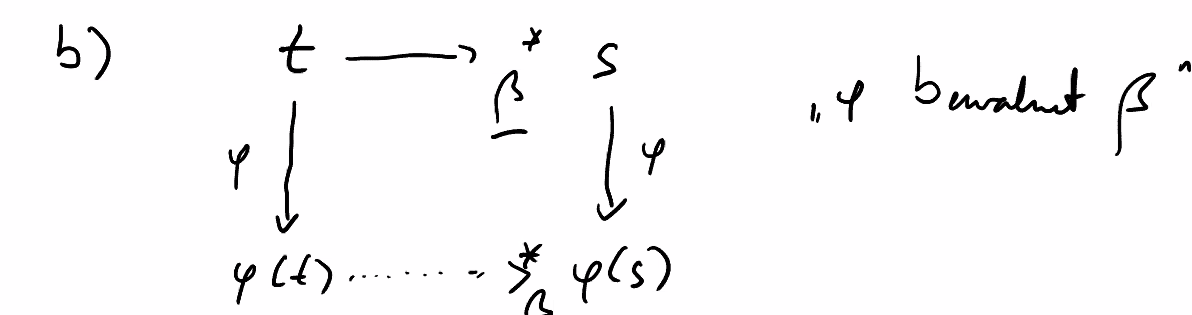
\includegraphics[width=256px]{images/LemmaB.png}\\
	\end{lemma}

	\begin{beweis}. \\
	a) Induktion über t, interessant nur $t=(\underline{\lambda}y.u)v$\\
	$\phi(((\underline{\lambda}y.u)v)[s/x])\stackrel{(1)}{=}\phi((\underline{\lambda}y.u[s/x])v[s/x]) = \phi(u[s/x])[\phi(v[s/x])/y]\\
	\stackrel{IV}{=} \phi(u)[\phi(s)/x][\phi(v)[\phi(s)/x])/y]\\
	\stackrel{synt.Subst+(1)}{=} \underbrace{\phi(u)[\phi(v)/y]}_{\phi((\underline{\lambda}y.u)v)}[\phi(s)/x]\\
	= \phi((\underline{\lambda}y.u)v)[\phi(s)/x]$\\
	 (1) o.E. $y\neq x$ $y\notin FV(s)$ ( im zweifelsfall umbennenen)\\
	b) Reduziere auf $t\to_{\underline{\beta}} s$, Induktion über Kontexte:\\
	$(\cdot):$ Fälle nach Markierung:\\
	Fall 1: markiert:\\
	$\begin{bmatrix} (\underline{\lambda}x.u)v&\to_{\underline{\beta}}& u[v/x]\\
	\phi&&\phi\\
	\phi(u)[\phi(v)/x]&=&\phi(u)[\phi(v)/x]
	\end{bmatrix}$\\
	Fall 2: unmarkiert:\\
	$\begin{bmatrix} (\lambda x.u)v&\to_{\underline{\beta}}& u[v/x]\\
	\phi&&\phi\\
	\lambda x.\phi(u)\phi(v)&\to_\beta&\phi(u)[\phi(v)/x]
	\end{bmatrix}$\\
	Beispiel mit nichtleerem kontext:\\
	Kontext $(\underline{\lambda} x.C(\cdot))s$ und $t\to_\beta s$\\
	$\phi(\underline{\lambda} x.C(t))s = \phi(C(t))[\phi(s)/x]\stackrel{IV, C\ ist\ kleinerer\ Kontext}{\to_\beta^*}\phi(C(s))[\phi(s)/x]\checkmark$
	\end{beweis}

	\begin{lemma} Lemma C\\
	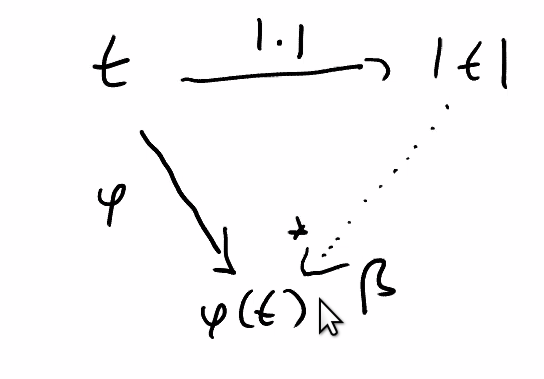
\includegraphics[width=256px]{images/LemmaC.png}\\
	\end{lemma}
	\begin{beweis} Induktion über t, interessanter Fall $t=(\underline{\lambda}x.u)v$ (sonst passiert ja nichts):\\
	$\begin{bmatrix}(\underline{\lambda}x.u)v&\tomark& (\lambda x.|u| )|v|\\
	\phi & &\phi\\
	\phi(u)[\phi(v)/x]&_\beta\leftarrow&(\lambda x.\phi(u))\phi(v)
	\end{bmatrix}$
	\end{beweis}
	$C((\lambda x.u)v)$\\
	\includegraphics[width=256px]{images/LambdaZusammenführung.png}\\
	\section{Curry-Howard Isomorphismus}
	Typen = Propositionen (=Formel) ``Types are propositions''.\\
	Terme/Programme = Beweise (u.U. ist ein Typ nicht bewohnt, also nicht Beweisbar)\\
	Coq ``man hat einen Term definiert, der diesen Typ hat''\\
	\underline{minimale Logik:} 
	\[\phi,\psi::= a|\phi\to\psi\; (a\in V)\]
	Deduktion:\\
	\AxiomC{$\phi\to\psi$}
	\AxiomC{$\phi$}
	\LeftLabel{$(\to_E)$}
	\BinaryInfC{$\psi$}
	\DisplayProof\\
	\AxiomC{$[\phi]\vdash\psi$}
	\LeftLabel{$(\to_I)$}
	\UnaryInfC{$\phi\to\psi$}
	\DisplayProof\\
	Sequenzenkalkül: $\underbrace{\Gamma}_{Menge Formeln}^{Annahme}\vdash \underbrace{\phi}_{Formel}$
	``linke Regel'' $(\to_E)$\\
	\AxiomC{$\Gamma \vdash \phi\to\psi$}
	\AxiomC{$\Gamma \vdash \phi$}
	\LeftLabel{$(\to_E)$}
	\BinaryInfC{$\Gamma\vdash \psi$}
	\DisplayProof\\
	\AxiomC{$\Gamma,\phi \vdash \psi$}
	\LeftLabel{$(\to_I)$}
	\UnaryInfC{$\Gamma\vdash \phi\to\psi$}
	\DisplayProof\\
	\AxiomC{}
	\LeftLabel{$(Ax)$}
	\UnaryInfC{$\Gamma\vdash \phi$}
	\DisplayProof\\
	\begin{satz} C-H-I:\\
	$\vdash \phi\iff \phi$ bewohnt\\
	\end{satz}
	\begin{beweis}. \\
	$\impliedby$ trivial: lösche Terme aus Herleitung von $\vdash t:\phi$ ergibt Herleitung $\vdash \phi$ (damit erhält man die kombination der $\phi$ als typen, dies sind trivialerweise die Herleitung)\\
	$\implies$ Zu $\Gamma$ definiert Kontext $\bar\Gamma$:\\
	$\Gamma =\{\phi_1,\dots,\phi_n\}\implies \bar\Gamma =\{x_1:\phi_1,\dots,x_n:\phi_n\}$\\
	Also jeder Term wird als Typ gewertet und bekommt eine Variable.\\
	Zeige $\Gamma\vdash \psi\implies \exists t(\bar\Gamma\vdash t:\psi)$\\
	per Induktion über Herleitungen von $\Gamma\vdash\psi$\\
	(Ax): $\phi\in\Gamma\implies \psi=\phi_i$ für ein $x_i:\phi_i\in\bar\Gamma \stackrel{(AX)}{\implies} \bar\Gamma \vdash x_i:\phi_i$\\
	$(\to_E)$\\
	\AxiomC{$\Gamma\vdash \phi\to\psi$}
	\AxiomC{$\Gamma\vdash \phi$}
	\LeftLabel{$(\to_E)$}
	\BinaryInfC{$\Gamma\vdash \psi$}
	\DisplayProof\\
	I.V. haben t,s mit\\
	\AxiomC{$\bar\Gamma\vdash t:\phi\to\psi$}
	\AxiomC{$\bar\Gamma\vdash s:\phi$}
	\BinaryInfC{$\bar\Gamma\vdash ts:\psi$}
	\DisplayProof\\
	($\to_I$) Beweis\\
	\AxiomC{$\Gamma,\phi\vdash\psi$}
	\LeftLabel{$(\to_I)$}
	\UnaryInfC{$\Gamma\vdash\psi\to\phi$}
	\DisplayProof\\
	I.V. haben (bei $\phi=\phi_{n+1}$)\\
	\AxiomC{$\bar\Gamma,x_{i+1}:\phi_{i+1}$}
	\AxiomC{$\vdash t:\psi$}
	\LeftLabel{$(\to_I)$}
	\BinaryInfC{$\bar\Gamma\vdash \lambda x_i.t:\phi_{i+1}\to\psi$}
	\DisplayProof\\
	\end{beweis}
	\textbf{\danger ``$\to$'' ist intuitionistisch!}\\
	z.B. $((a\to b)\to a)\to a$ ist klassisch gültig, aber in miminaler (intuitionistischer) Logik nicht herleitbar.\\
	\AxiomC{}
	\LeftLabel{(Ax)}
	\UnaryInfC{$(a\to a)\vdash (a \to a)\to a$}
	\AxiomC{}
	\LeftLabel{(Ax)}
	\UnaryInfC{$(a\to a)\to ,a \vdash a$}
	\UnaryInfC{$(a\to a)\to a\vdash a \to a$}
	\LeftLabel{$(\to_E)$}
	\BinaryInfC{$(a\to a) \to a\vdash a$}
	\LeftLabel{$(\to_I)$}
	\UnaryInfC{$\vdash((a\to a\to) a)\to a$}
	\DisplayProof\\
	Auf Typebene:\\
	$\underbrace{((a\to a)\to a)\to a}_{\lambda f.f(\lambda x.x)}$\\
	Man hat eine funktion, die wieder eine funktion erhält also das innere $(a\to a)\to a$ und hat als Ergebnis wieder ein a. Dazu muss man anwenden. Die innerer funktion muss den typ $a\to a$ haben. Das einzig mögliche hierfür ist die identitätsfunktion $\lambda x.x$\\
	Deshalb haben wir eine funktion f in den wir eine funktion (identität) haben.\\
	\section{Induktive Datentypen}
	\begin{minted}{haskell}
	data Nat where
		0: ()-> Nat
		Suc: Nat->Nat
	\end{minted}
	definiert Signatur $\Sigma_{Nat} = \{0/0,Suc/1\}$\\
	Die Semantik von Nat ist definiert als\\
	$\llbracket Nat\rrbracket=\{0,Suc(0),Suc(Suc(0)),\dots\}$ also ein Herbrandmodell.\\
	\begin{definition} Ein $\Sigma$-Modell ($\Sigma$-Algebra) $\mathfrak{M}$ besteht aus\\
	\begin{itemize}
		\item Menge M (Träger)
		\item zu f/n$\in\Sigma$
		\item $\mathfrak{M}\llbracket f\rrbracket:M^n\to M$
	\end{itemize}
	Interpretion von Termen unter \underline{Umgebung} $\eta:V\to M:$\\
	\[\mathfrak{M}\llbracket t\rrbracket\eta \in M\]
	\[\mathfrak{M}\llbracket x\rrbracket\eta= \eta(x)\; x\in V\]
	\[\mathfrak{M}\llbracket f(t_1,\dots,t_n)\rrbracket\eta= \mathfrak{M}\llbracket f\rrbracket(\mathfrak{M}\llbracket t_1\rrbracket\eta,\dots,\mathfrak{M}\llbracket t_n\rrbracket\eta)\]
	\end{definition}
	\newcommand{\dbrack}[1]{\llbracket #1\rrbracket}
	\begin{beispiel} $\dbrack{Nat}$ ist eine $\Sigma_{Nat}$-Algebra per:\\
	\[\dbrack{Nat}\dbrack{0} = 0\]
	\[\dbrack{Nat}\dbrack{succ}(x) = Suc(x)\in\dbrack{Nat}\]
	\end{beispiel}
	\begin{definition} Seien $\mathfrak{M},\mathfrak{N}\; \Sigma$-Algebren.\\
	$\Sigma-$Homomorphismus = Abbildung $h:M\to N$ (wobei M,N trägermengen des respektiven Models sind)\\
	$\forall f/n \in \Sigma, x_1,\dots, x_n\in M$
	\[h(\mathfrak{M}\dbrack{f}(x_1,\dots,x_n)) = \mathfrak{N}\dbrack{f}(h(x_1),\dots,h(x_n))\]
	Erinnerung: lineare Abbildung:
	\[ h(\lambda \cdot x) = \lambda h(x)\land h(x+y)=h(x)+h(y)\]
	sprich: homomorphismen sind lineare Abbildung zwischen Algebren.\\
	\end{definition}
	\begin{lemma} 
	\begin{itemize}
		\item $id_n:\mathfrak{M}\to\mathfrak{M}$ ist $\Sigma$-Homomorphismus
		\item $h:\mathfrak{M}\to\mathfrak{N}, k:\mathfrak{N}\to\mathfrak{P}$ sind $\Sigma$-Homomorphismus$ \implies k\cdot h:\mathfrak{M}\to\mathfrak{P}$ ist $\Sigma$-Homomorphismus
	\end{itemize}
	\end{lemma}
	\begin{definition} h ist isomorphismus $\iff$ h $\Sigma$-Homomorphismus und bijektiv.\\
	$\iff \exists h^{-1}(h\cdot h^{-1}=id\land h^{-1}\cdot h=id)$ (aber i.A. zwei verschiedene identitätsfunktionen!)\\
	Isomorphismen sind also strukturerhaltend!!!\\
	Dies gilt nicht in jedem Kontext: geordnete Systeme lassen das nicht einfach so zu!.\\
	Menge A $\{b,\gamma\}$ ohne Ordnung und eine geordnete Menge B $(\{1,0\},\leq)$.\\
	Es gibt ein $h:A\to B: x\leq y\implies h(x)\leq h(y)$\\
	Aber das $h^{-1}$ ist nicht monoton: $0\leq 1, h^{-1}(0)\nleq h^{-1}(1)$\\
	Das heißt die Abbildung die im Algebraischen sinne isomorphismen sind, sind nicht unbedingt isomorphismen im Kontext der geordneten Mengen.
	\end{definition}
	\begin{lemma} h Isomorphismus $\implies h^{-1}$ ist Isomorphismus
	\end{lemma}
	\begin{beweis} zZ: $h^{-1}$ ist Homomorphismus (bijektivität ist ja bereits bekannt!), d.h.\\
	$h^{-1}(\mathfrak{N}\dbrack{f}(y_1,\dots,y_n)=\mathfrak{M}\dbrack{f}(h^{-1}(y_1),\dots,h^{-1}(y_n)))\stackrel{h\ injektiv}{\iff} \underbrace{h(h^{-1}(\mathfrak{N}\dbrack{f}(y_1,\dots,y_n)) }_{\mathfrak{N}\dbrack{f}(y_1,\dots,y_n)}= \underbrace{h(\mathfrak{M}\dbrack{f}(h^{-1}(y_1),\dots,h^{-1}(y_n))))}_{=\mathfrak{N}\dbrack{f}(h(h^{-1}(y_1)),\dots,h(h^{-1}(y_n)))}$
	\end{beweis}
	Erinnerung $m\equiv n (mod 4)$ ist Äquivalenzklasse $\mathbb{Z}/4\mathbb{Z} = \{[n]_4|n\in\mathbb{Z}\} = \{[0]_4,[1]_4,[2]_4,[3]_4\}$\\
	Darauf kann addition definiert werden: $[n]_4 +[m]_4 = [n+m]_4$ ist wohldefiniert.\\
	\begin{beispiel} $\Sigma_{Nat}$-Algebra $\mathfrak{M}$ mit $M=\mathbb{Z}/4\mathbb{Z},\mathfrak{M}\dbrack{0} = [0]_4, \mathfrak{M}\dbrack{suc}([n]_4) = [n+1]_4$\\
	$h:\dbrack{Nat}\to \mathfrak{M}$\\
	$Suc^n(0)\mapsto [n]_4$ ist homomorph:\\
	$h(\dbrack{Nat}\dbrack{0}) = [0]_4 =\mathfrak{M}\dbrack{0}$\\
	$h(\dbrack{Nat}\dbrack{Suc}(Suc^n(0)))=h(Suc^{n+1}(0)) = [n+1]_4 =\mathfrak{M}\dbrack{suc}([n]_4)=\mathfrak{M}\dbrack{Suc}(h(Suc^n(0)))$ (sogar surjektiv homomorph, aber natürlich nicht injektiv, somit kein isomorphismus)
	\end{beispiel}
	Allg.: Datentyp D= Signatur $\Sigma$, $\dbrack{D} = \dbrack{\Sigma} = T_\Sigma (\emptyset)$ (also alle geschlossenen Terme) als Algebra, mit $\dbrack{\Sigma}\dbrack{f}(t_1,\dots,t_n) = f(t_1,\dots, t_n)$\\
	\begin{definition} $\Sigma-$Algebra $\mathfrak{M}$ initial $\iff\forall \mathfrak{N}\ \exists!\ Homomorphismus\ h:\mathfrak{M}\to\mathfrak{N}$ (initiales Modell ist also algemeinstes Modell)
	\end{definition}
	\begin{satz} $\dbrack{\Sigma}$ ist initial genannt ``Termalgebra''\end{satz}
	\begin{beweis} Sei $\mathfrak{N}$ eine $\Sigma$-Sigma Algebra. zZ: $\exists! h$ mit 
	\[(*)\ h(\dbrack{\Sigma}\dbrack{f}(t_1,\dots,t_n))=\mathfrak{N}\dbrack{f}(h(t_1),\dots,h(t_n))\; (f/n\in\Sigma)\]
	gilt für $h(t)=\mathfrak{N}\dbrack{t}$,\\
	(*) ist rekursive Definition von $\mathfrak{N}\dbrack{\dots}$
	\end{beweis}
	\begin{satz} Die initiale $\Sigma$-Algebra ist eindeutig bis auf \textbf{eindeutige} Isomorphie (also kategorietheorie\dots)
	\end{satz}
	\begin{beweis} Seien $\mathfrak{M},\mathfrak{N}$ initial\\
 	\[\mathfrak{M} \stackanchor{$\exists ! h\to$}{$\gets\exists! k$}\mathfrak{N}\]
	Zu $\mathfrak{M},\mathfrak{N}$ gehört jeweils eine identitätsfunktion.\\
	Wegen eindeutigkeit der homomorphismen, muss $k\cdot h=id$ sein (bzw $h\cdot k=id$)\\
	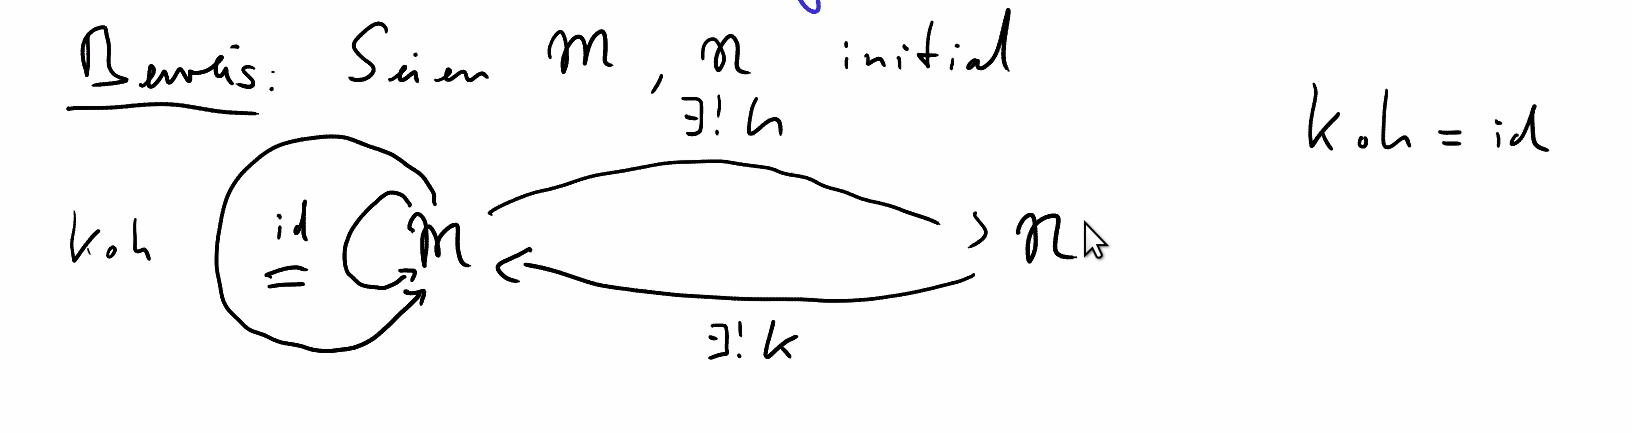
\includegraphics[width=256px]{images/initialEindeutigkeit.png}\\
	technisch gesehen definiert sich damit eine Äquivalenzklasse über $\Sigma$-Algebraen.\\
	\end{beweis}
	\subsection{Mengenkonstruktionen}
	$X_1,X_2$ Mengen $X_1\times X_2=\{(x_1,x_2)|x_1\in X_1, x_2\in X_2\}$\\
	$\pi_i(x_1,x_2) = x_1$ (i-te Projektion, i=1,2)\\
	$\pi_i : X_1\times X_2 \to X_i$\\
	Mehrer funktionen auf gleiche daten:\\
	$f_i: Y\to X_i$ (i=1,2)\\
	$<f_1,f_2>:Y\to X_1\times X_2$\\
	$y\mapsto (f_1(y),f_2(y))$\\
	kartesisches Produkt von Projektionen. (lifting)\\
	$g_i: Y_i\to X_i$\\
	$g_1\times g_2 :Y_1\times Y_2\to X_1\times X_2$\\
	$(y_1,y_2)\mapsto (g_1(y_1),g_2(y_2))$\\
	Beispiele:\\
	$\pi_i\cdot <f_1,f_2> = f_i$\\
	$<\pi_1,\pi_2> = id$, $<\pi_1\cdot f, \pi_2\cdot f> =f$\\
	$g_1\times g_2 = <g_1\cdot \pi_1, g_2\cdot \pi_2>$\\
	$X_1+X_2$ (addition als analog zur Multiplikation mit kartesischen produkt)\\
	\[X_1+X_2 = \{(i,x)|i\in\{1,2\}, x\in X_i\}\]
	(umbennen, damit keine zwei elemente sich gegenseiteig in der Menge auslöschen)
	Duale\\
	$X_i\to X_1+x_2$\\
	$x\mapsto (i,x)$\\
	zu $f_i:X_i\to Y\ (i=1,2)$\\
	kopaar.\\
	$[f_1,f_2]:X_1+X_2\to Y$\\
	$[f_1,f_2](i,x)\mapsto f_i(x)$ (man wählt also die i-te funktion aus. effektiv ``case'' statement)\\
	zu $g_i:X_i\to Y_i\ (i=1,2)$\\
	$g_1+g_2: X_1+X_2\to Y_1+Y_2$\\
	$(g_1+g_2)(i,x)\mapsto (i,g_i(x))$\\
	\begin{lemma} Duale:\\
	$[f_1,f_2]\circ in_i=f_i$\\
	$r\circ in_1, r\circ in_2] = r$ \\
	$g_1+g_2 = [in_1\circ g_1, in_2\circ g_2]$
	\end{lemma}
	\begin{beweis}
	$[f_1, f_2](in_i(x))=[f_1,f_2](i,x) = f_i(x)$\\
	$[r\circ in_1, r\circ in_2](i,x)= r(in_i(x)) = r(i,x)$\\
	$[in_1\circ g_1, in_2\circ g_2](i,x) = in_i(g_i(x)) = (i,g_i(x)) = (g_1+g_2)(i,x)$
	\end{beweis}
	\begin{beispiel} Bäume\\
	\begin{minted}{haskell}
	data Tree where
		Nil: ()-> Tree
		Node: Tree*Tree->Tree
	\end{minted}
	Eine $\Sigma_{Tree}$-Algebra $\mathfrak{M}$:\\
	$\mathfrak{M}\dbrack{Nil}: 1\to M$ (wobei 1 unit $\{*\}$ ist)\\
	$\mathfrak{M}\dbrack{Node}:M^2\to M$\\
	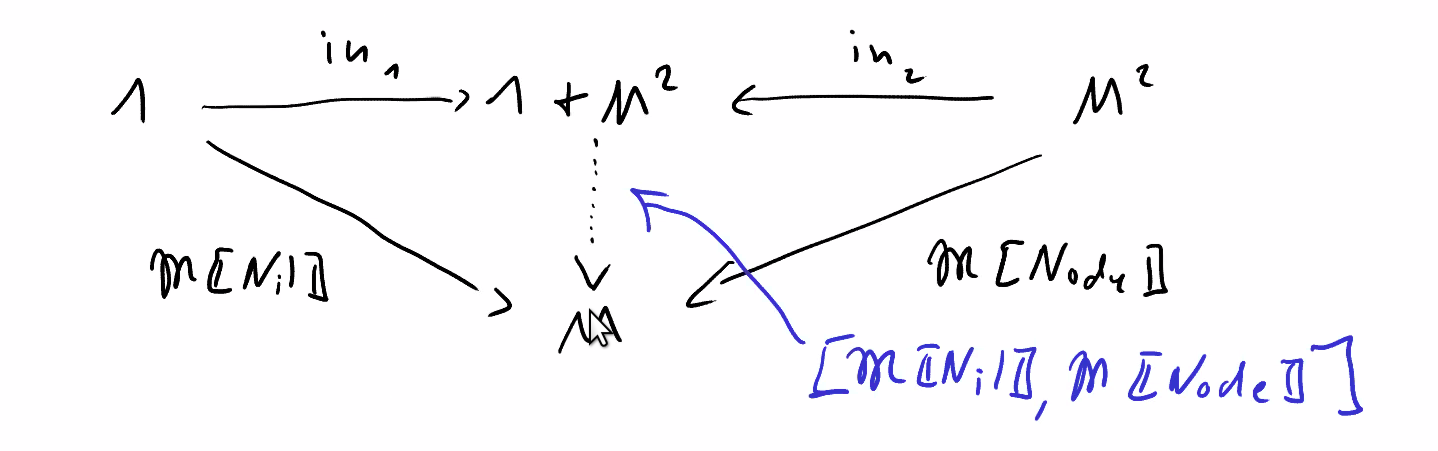
\includegraphics[width=256px]{images/TreeAlgebra.png}\\
	d.h. $\mathfrak{M}$ gegeben durch $\alpha:1+M^2\to M$\\
	($\mathfrak{M}\dbrack{Nil}=\alpha(in_1(*))$ und $\mathfrak{M}\dbrack{Node}=\alpha(in_2(x,y))$)\\
	h homomorph bezüglich Node $\iff h(\mathfrak{M}\dbrack{Node}(x,y)) = \mathfrak{N}\dbrack{Node}(h(x),h(y))$\\
	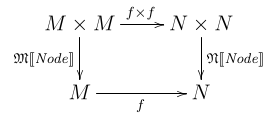
\includegraphics[width=256px]{images/TreeHomomorphism.png}\\
	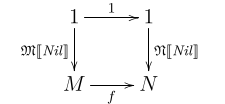
\includegraphics[width=256px]{images/TreeHomomorphismNil.png}\\
	\includegraphics[width=256px]{images/VollständigTreeHomomorphism.png}\\
	Erinnerung die Eckigen klammern heißen: gib mir vom paar $[f_1, f_2](i,x)$ die i-te funktion angewandt auf x.\\
	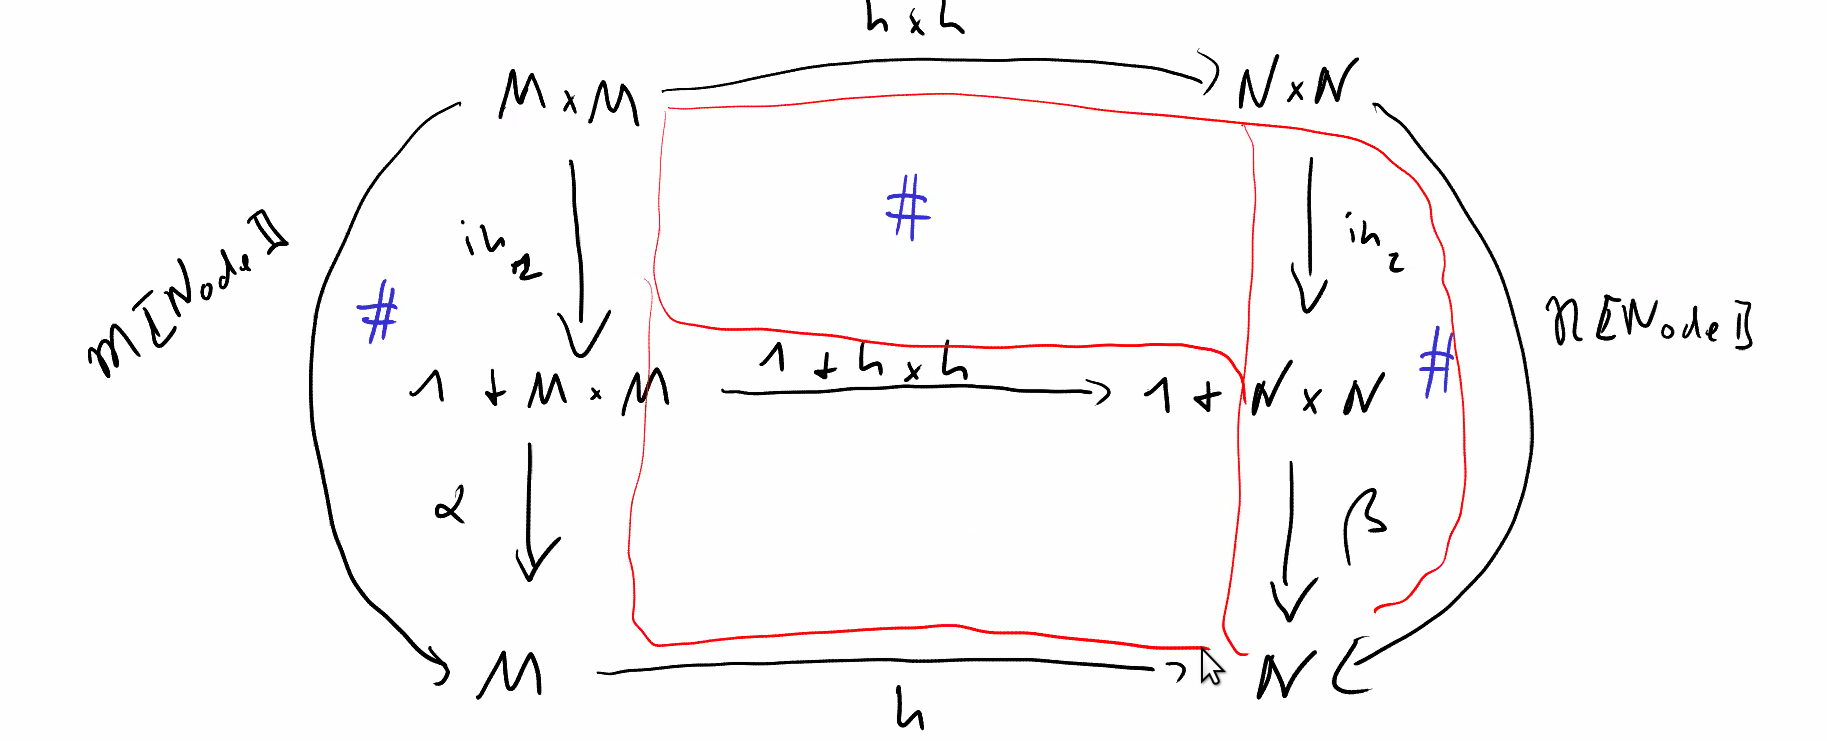
\includegraphics[width=256px]{images/kommutationTree.png}\\
	Da jedes Teildiagram kommutiert, gilt homomorphie.\\
	(Das gilt genau so für NIL (wenn man $in_2$ verwendet))\\
	\end{beispiel}
	Allgemein gilt für eine $\Sigma$-Algebra 
	\[= \alpha:\sum_{\underbrace{f/n\in\Sigma}_{=: F_\Sigma M}} M^n\to M\]
	Dann $h\mathfrak{M}\to\mathfrak{N}$ Homomorphismus $\iff$ $F_\Sigma$\\
	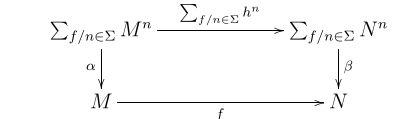
\includegraphics[width=256px]{images/allgHomomorphismus.png}\\
	sprich, wenn man für alle signatursymbole $f$ ein solches signaturquadrat bauen kann, dann gilt homomorphismus. ($F_\Sigma h=\sum_{f/n\in\Sigma} h^n$)\\
	Man kann also alles in eine Abbildung darstellen: das h wird einfach der Tuple aller homomorphismen eines signatursymbole!
	\subsection{Initialität und Rekursion}
	Datentyp $\Sigma:\dbrack{\Sigma}$ Initiale $\Sigma$-Algebra.\\
	zu $f/n$ wähle $a_f: A^n\to A$ (konstruktion einer Algebra zu $\Sigma$)\\
	Dan existiert ein eindeutiger homomorphismus (per def. der initialität) $h:\dbrack{\Sigma}\to A$ mit
	\[h(\underbrace{f(\underbrace{x_1,\dots,x_n}_{konstruktorargumente})}_{konstruktorpattern}) = a_f(\underbrace{h(x_1),\dots, h(x_n)}_{rekursive\ Aufrufe\ von\ h})\]
	Rekursive Definition von h (definiert eindeutig h) also $a_f$ sind irgendwelche funktionen, die etwas vom typ A liefern. (man wechselt also von $\dbrack{\Sigma}$ auf A mithilfe eines homomorphismus)\\
	man nennt dies das \textbf{fold-Schema}: h= fold ($\lambda y\dots y_n. a_f)_{f\in\Sigma}$ (sprich $a_f$ ist eine totale funktion über f.)\\
	z.B. Tree: $(fold c g):Tree\to a$ mit $c:a, g:a\to a\to a$\\
	\begin{minted}{haskell}

	fold c g Nil = c
	fold c g (Node x y) = g (fold c g x) (fold c g y)
	-- sprich man baut hier ein pattern auf, dass einmal eine interpretation a_NIL =c
	-- und eine interpretation a_Node(x,y) = g erwartet
	\end{minted}
	fold 1 * = $\lambda x.1$ (also multiplikation aller blätter, wobei jedes blatt wert 1 hat)\\
	fold 1 + = $\lambda x.\#leaves(x)$\\
	\begin{minted}{haskell}
	fact 0 = 1
	fact (suc n) = (suc n)*(fact n)
	--problem man braucht auch suc n, nicht nur das ergebnis des rekursiven aufrufs fact!
	\end{minted}
	Dies kann man jedoch lösen:\\
	$h=<fact,id>$ wenn man das programmieren kann, dann kann man das im fold schema schreiben, da in h ja die id drinnen ist.
	\begin{minted}{haskell}
		h 0 = (1,0)
		h (suc n) = (( succ (snd (h n) )) *(fst (h n)), suc (snd (h n)))
		-- snd ist das selbe wie die 2.projektion pi_2
	\end{minted}
	Mehrstellige Funktionen:\\
	$+: Nat\times Nat\to Nat$\\
	\begin{minted}{haskell}
	0+k=k
	(suc n)+k = suc (n+k)
	\end{minted}
	Currying: $+:Nat\to (Nat\to Nat)$\\
	$+ = fold (\lambda k.k) \underbrace{(\lambda fk.Suc (f\ k))}_{(Nat\to Nat)\to (Nat\to Nat)}$
	primitive Rekursion:\\
	Rekursion über Argumente verwende rekursive Aufrufe auf Konstruktorargumente.\\
	\subsection{Mehrsortige Typen}
	\begin{minted}{haskell}
	data Tree a, Forest a where
		Leaf: a-> Tree a
		Node: Forest a-> Tree a
		Nil: ()-> Forest a
		Cons: Tree a * Forest a-> Forest a
		-- bzw Cons:Tree a->Forest a-> Forest a
	\end{minted}
	mehrsortige Signatur, hier Sortenmenge $S=\{\underbrace{a}_{S_0},Tree\ a, Forest\ a\}$\\
	\begin{definition} Eine sortierte Signatur $\Sigma=(S_0, S,F)$ besteht aus:\\
	\begin{itemize}
		\item Einer Menge S von Sorten
		\item Menge $S_0\subseteq S$ von Parametern
		\item Eine Menge F von Funktionssymbolen bzw. Konstruktoren c mit \underline{Profilen} $c:a_1\times\dots\times a_n\to b$ mit $n\geq 0$ $a_1,\dots,a_n\in S$ und $b\in S\setminus S_0$ (sprich wir das ziel soll nicht wieder ein Parameter sein $Tree\ a\to Forest\ a$)
	\end{itemize}
	\end{definition}
	\begin{definition}.\\
	\begin{itemize}
		\item Ein Kontext ist eine Menge $\Gamma = \{x_1:a_1,\dots,x_k:a_k\}$ mit Sorten $a_i\in S$ paarweise verschiedenen Variablen $x_i$. (also endliche partielle Abbildung $\Gamma: Var\to Sorte$)
		\item $\Gamma\vdash t:a$ ``Term t hat im Kontext $\Gamma$ Sorte a''
	\end{itemize}
	definier induktiv:\\
	\AxiomC{}
	\RightLabel{$(x:a\in \Gamma)$}
	\UnaryInfC{$\Gamma\vdash x:a$}
	\DisplayProof\\
	\AxiomC{$\Gamma \vdash t_1:a_1,\dots \Gamma\vdash t_n:a_n$}
	\RightLabel{$(c:a_1\times\dots\times a_n\to b)$}
	\UnaryInfC{$\Gamma\vdash c(t_1,\dots,t_n):b$}
	\DisplayProof\\
	Wir schreiben $T_\Sigma(\Gamma)_a = \{t\ Term|\Gamma\vdash t:a\}$ für die Menge der Terme der Sorte a im Kontext $\Gamma$.\\
	z.B. $x:a\vdash Node (Cons\ (Node\ Nil)\ (Cons(Leaf\ x) Nil)):Tree\ a$
	\end{definition}
	\begin{definition} Sei $V=(V_a)_{a\in S_0}$ eine Mengenfamilie. Eine mehrsortige $\Sigma$-Algebra $\mathfrak{M}$ über V besteht aus\\
	\begin{itemize}
		\item für $a\in S$ Menge $\mathfrak{M}\dbrack{a}=V_a$
		\item einer Abbildung
	\end{itemize}
	$\mathfrak{M}\dbrack{c}:\mathfrak{M}\dbrack{a_1}\times\dots\times \mathfrak{M}\dbrack{a_n}\to \mathfrak{M}\dbrack{b}$\\
	für jedes $c:a_1\times\dots\times a_n\to b$\\
	Gegeben $\mathfrak{M}$ Umgebung $\eta$ für $\Gamma$ (d.h. $\eta(x)\in\mathfrak{M}\dbrack{a}$ für jede $\Gamma(x)=a$), $\Gamma\vdash t:a$
	\[\mathfrak{M}\dbrack{t}\eta\in\mathfrak{M}\dbrack{a}\]
	rekursiv definiert wie bisher.\\
	\end{definition}
	Ein \underline{$\Sigma$-Homomorphismus}	$h:\mathfrak{M}\to \mathfrak{N}$ über V besteht aus Abbildungen (ist also selbst mehrsortig)
	 \[h_a:\mathfrak{M}\dbrack{a}\to\mathfrak{N}\dbrack{a}\ (a\in S)\]
	mit $h_a=id$ für $a\in S_0$ (Parameter werden in ruhe gelassen)\\
	sodass
	\[h_b(\mathfrak{M}\dbrack{c}(x_1,\dots,x_n)) = \mathfrak{N}\dbrack{c}(h_{a_1}(x_1),\dots,h_{a_n}(x_n))\]
	für $c:a_1\times \dots\times a_n\to b\in\Sigma$\\
	\underline{Termalgebra}\\
	Zu $V=(V_a)_{a\in S_0}$ setze $\Gamma(V)=\{x:a|a\in S_0,x\in V_a\}$\\
	Termalgebra $\dbrack{\Sigma}_V$ (Semantik des Datentyps $\Sigma$ gegeben V)
	\[\dbrack{\Sigma}_V\dbrack{a} = T_\Sigma(\Gamma(V))_a\  (a\in S)\]
	\[\dbrack{\Sigma}_V\dbrack{c}(t_1,\dots, t_n) = c(t_1,\dots t_n)\]
	\begin{satz} Initialität/Fold-Prinzip\\
	Für jede $\Sigma$-Algebra $\mathfrak{N}$ über V existiert genau ein $\Sigma-$Homomorphismus
	\[h:\dbrack{\Sigma}_v\to \mathfrak{N}\]
	über V. (Termauswertung $\eta(x)=x$), sonst wie vorher\\
	$\underbrace{fold (Algebra):}_{mehrere\ Abbildungen!} \dbrack{\Sigma}_V\to\dots$
	\end{satz}
	\begin{beispiel} $\Sigma_{Tree}$-Algebra $\mathfrak{N}$ über $V_a = \mathbb{N}$ (es gab hier ja nur eine\dots)
	$\mathfrak{N}\dbrack{Tree\ a}=\mathbb{N}=\mathfrak{N}\dbrack{Forest\ a}$ (also hier forest und tree gleich interpretation)
	$\mathfrak{N}\dbrack{Leaf}(n)=n$\\
	$\mathfrak{N}\dbrack{Node}(n)=n$\\
	$\mathfrak{N}\dbrack{Cons}(n,m)=n+m$\\
	$\mathfrak{N}\dbrack{Nil}=0$\\
	primitive Rekursion (gegenseitig) \danger Alle interpretationen müssen auf ein mal definiert werden!\\
	\subsection{Strukturelle Induktion über Datentypen}
	\begin{minted}{haskell}
	data List a where
		Nil:()->List a
		Cons: a->List a-> List a
	concat::List a->List a-> List a
	concat Nil k=k
	concat (Cons x l) k = Cons x (concat l k)
	\end{minted}
	Beweisen Assoziativität:
	cc l (cc k v) = cc ((cc l k) v)\\
	Strukturelle Induktion: Ein Fall pro Konstruktor \\
	I.V. jeweils für Konstruktorargumente (also immer induktion über das argument, dass auch rekursion betreibt)\\
	hier über l\\
	-Nil: cc Nil (cc k v) = cc k v = cc ( cc Nil k) v\\
	Cons: cc (Cons x l) (cc k v) = Cons x (cc l (cc k v)) $\stackrel{=}{IV}$ Cons x (cc ( cc l k) v) = cc ( cc (cons x l) k) v = cc (Cons x (cc l k)) v = Cons x (cc ( cc l k) v)
	\end{beispiel}
	\subsection{strukturelle Induktion über mehrsortige Datentypen}
	\begin{minted}{haskell}
	mirrort::Tree a->Tree a
	--wald an senkrechter achse spiegeln, also wald und jeden baum an einer senkrechten achse spiegeln
	mirrorf::Forest a->Forest a
	mirrort (Leaf x) = Leaf x
	mirrort (Node f) = Node (mirrorf f)
	mirrorf Nil = Nil
	mirrorf (Cons t f) = concat (mirrorf f) (Cons (mirror t) Nil)
	--sortiertes flattening nach baumreihenfolge
	flattent: Tree a->List a
	flattenf: Forest a->List a
	flattent (Leaf x) = [x]
	flattent (Node f) = flattenf f
	flattentf Nil = []
	flattenf (Cons t f)=  concat (flattent t) (flattenf f)
	rev:List a->List a
	rev Nil = Nil
	rev (Cons x y) = concat (rev y) [x]
	\end{minted}
	Behauptung: flattent (mirrort t) = rev (flattent t)\\
	Induktion über t:\\
	flattent (mirrort (Leaf x)) = [x] = rev (flattent (Leaf x))\\
	Leaf geht, Node:\\
	flattent (mirrort (Node f)) = flattent (Node (mirrorf f) ) = flattenf (mirrorf f)\\
	andere seite:\\
	rev ( flattent (Node f)) = rev ( flattenf f)\\
	Induktionsbehauptung für f:Forest a\\
	flattenf (mirrorf f) = rev (flattenf f)\\
	dann gilt ``rev ( flattenf f) =  flattenf (mirrorf f)'' per I.V.\\
	jetzt müssen wir die Induktionsvorraussetzung für Wälder anwenden: sprich dass flattenf (mirrorf f) = rev (flattenf f) für alle Wälder gilt\\
	flattenf (mirrorf Nil) = [] = rev (flattenf Nil)\\
	gilt also für Nil, jetzt Cons\\
	flattenf (mirrorf (Cons t f)) = flattenf (concat (mirrorf f) (Cons (mirror t) Nil)) $\stackrel{=}{Lemma\ A}$ concat (flattenf (mirrorf f)) (flattenf (Cons (mirrort t) Nil))
	$\stackrel{=}{Lemma\ B}$ concat ($\underbrace{flattenf (mirrorf\ f)}_{IV Forest}$) ($\underbrace{flattent (mirrort\ t))}_{IV Tree}$) = concat (rev (flattenf f)) (rev (flattent t))\\
	andere seite\\
	rev (flattenf (Cons t f)) = rev (concat (flattent t) (flattenf f))\\
	ist gleich (Vgl Übung, bzw umgekehrte concatenation von zwei invertierten listen ist gleich der invertierten list)\\
	\underline{Lemma A}: flattenf (concat f g) = concat (flattenf f) (flattenf g)\\
	Beweis: Induktion über f (aber hier haben wir keine Bäume!! I.A. für bäume könnte $T$ sein, der Beweis ist unabhängig). Trivial beweisbar via induktion.\\
	\underline{Lemma B}: flattenf [t] = flattent t (trivial, ausrechnen)\\
	flatten einfach als fold:\\
	fold $\lambda x.[x]$ id [] cc\\
	mirror als fold\\
	fold Leaf Node Nil $(\lambda x y.cc\ y [x])$\\
	das einzige, was bei mirror ``was macht'' ist Cons, bei dem werden die resultate der unteren schicht in umgekehrter Reihenfolge verbunden (und das erste zum forst ``casten'')
	\subsection{Kodaten}
	Daten werden konstruiert $Cons\ x\ Nil$\\
	Kodaten werden destruiert/beobachtet\\
	z.B. $A^\omega=\{a_0,a_1,a_2,\dots|a_i\in A\}$ streams über A. (omega als Menge der ordinale, für uns einfach Nat)\\
	hd (head): $A^\omega\to A$ gibt $a_0$ aus $a_0:a_1a_2\dots$ zurück.\\
	tl (tail): $A^\omega\to A^\omega$\\
	$(a_0,a_1,\dots)\mapsto (a_1,a_2,\dots)$\\
	\begin{minted}{haskell}
	codata Stream where
		hd:Stream->A
		tl:Stream->Stream
	\end{minted}
	Im gegensatz zu Datentypen, die über konstruktoren definiert ist, sind Kodatentypen über destructoren definiert.\\
	\begin{minted}{haskell}
	map f:Stream->Stream
	 hd(map f s) = f (hd s)
	 tl (map f s) = map f (tl s)
	\end{minted}
	Definition von map, allerdings terminiert map nie (soll es schließlich auch nicht).\\
	Zunächst $<hd,tl>:A^\omega\to A\times A^\omega$\\
	wir produzieren also aus $A^\omega$ eine ding aus der Trägermenge hinaus.(Destruction)\\
	Koalgebra: Träger M, Abb $\alpha:M\to A\times M$\\
	$A^\omega$ ist Koalgebra (genauer $(A^\omega,<hd,tl>)$ ist Koalgebra)\\
	weiter Koalgebra:\\
	$(A^\omega,<f\circ hd,tl>)$, denn $A^\omega\stackrel{hd}{\to}A\stackrel{f}{to}A$\\
	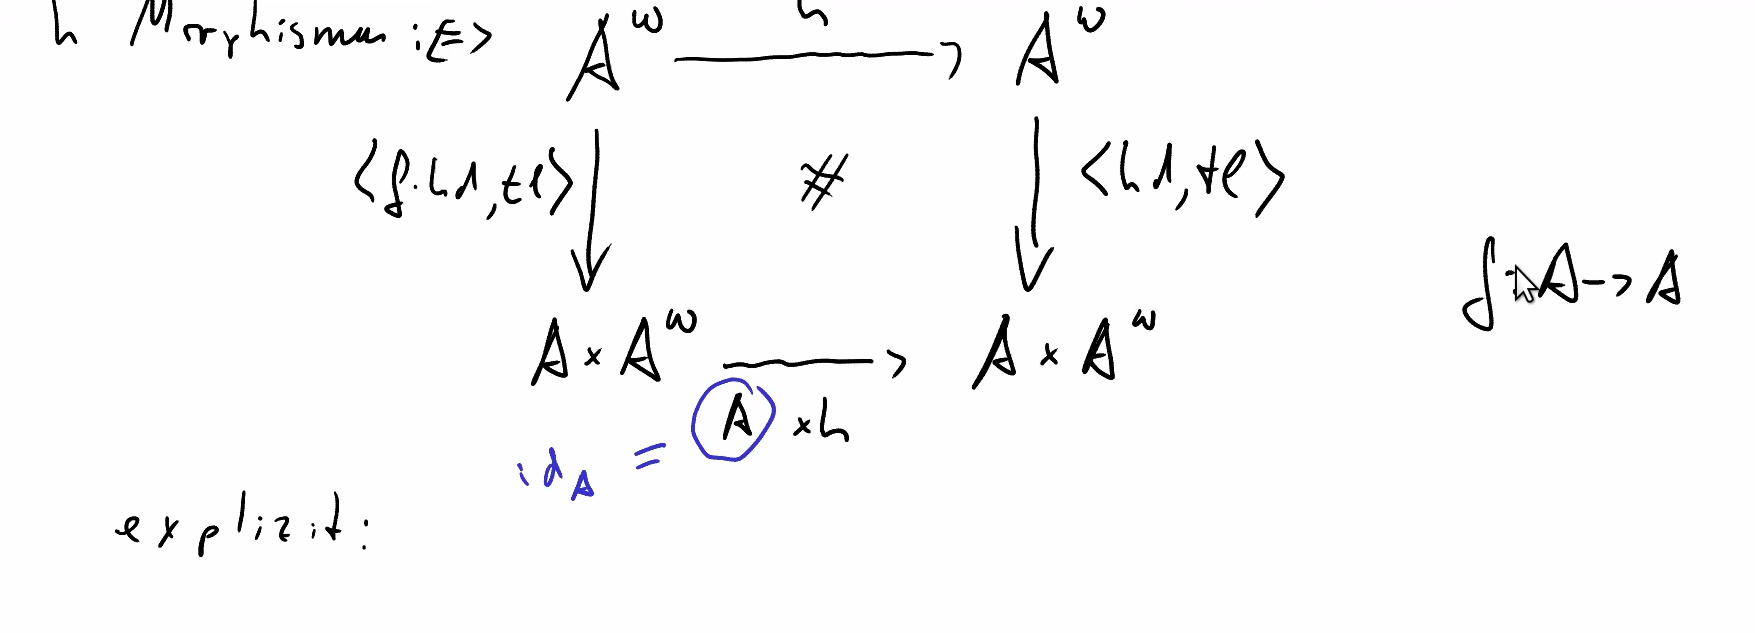
\includegraphics[width=256px]{images/CoalgebraHomomorph.png}\\
	explizit:\\
	linke Komponente: hd(h(s)) = f(hd(s))\\
	rechte Komponente: tl(h(s)) = tl(h(s))\\
	Mengenoperatoren: (polynomialfunktoren)\\
	$G::=A|id|(G_1+G_2)|G_1\times G_2$ A Menge (zum eingeklammerten werden wir nicht kommen)\\
	GX rekursiv definiert:\\
	$(A)X=A$\\
	$id(X)=X$\\
	$(G_1+G_2)X = G_1X+G_2X$\\
	$(G_1\times G_2)X = G_1X\times G_2X$\\
	entsprechend mit abbildungen Gf: $GX\to GY$ ($f:X\to Y$)\\
	\begin{definition} Eine \underline{G-Koalgebra}\\
	besteht aus einer Menge M (von ``Zuständen'') und Abbildung $\alpha:M\to GM$ (Transitionsabbildung, welche Zustände sind von M aus erreichbar und welche beobachtung).\\
	\end{definition}
	\begin{beispiel}.\\
	G=$A\times id$
	\end{beispiel}\noindent
	G-Koalgebra = Koalgebra oben:\\
	$M\to A\times M$\\
	Eine Koalgebra besteht aus 2 sub-abbildungen: $M\to A$ (``outputabbildung'') und $M\to M$ (``next-abbildung'') das kreuzprodukt aus beiden ist die Hauptabbildung.\\
	z.B. $A=\{a,b,c\}$\\
	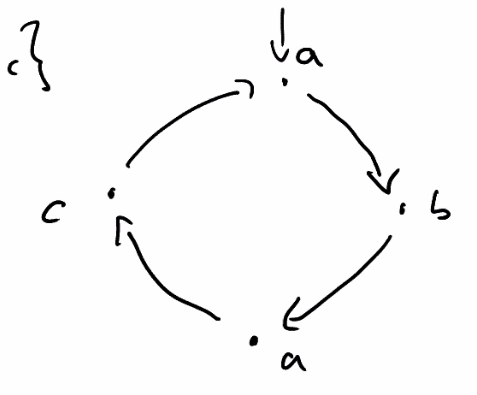
\includegraphics[width=256px]{images/GKoalgebra-AS-Statemachine.png}\\
	Stream abacab\dots\\
	G-Koalgebraen sind Dual zu den Koalgebra (sie haben ein ``unfold'' statt ein ``fold'' prinzip)\\
	\begin{definition} Ein (G-Koalgebra-)Morphismus zwischen G-Koalgebren $\alpha:M\to GM$ $\beta:N\to GN$ ist eine Abbildung $h:M\to N$ mit\\
	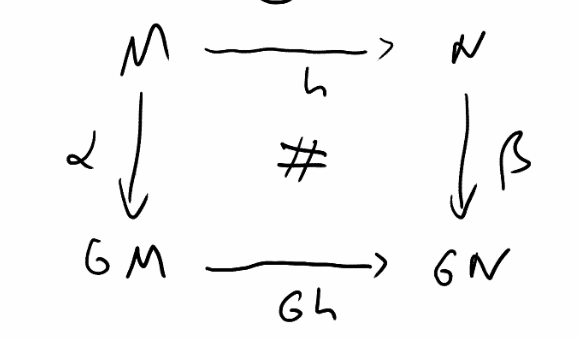
\includegraphics[width=256px]{images/G-Morphismus.png}\\
	$\alpha: M\to GM = A\times M = <\underbrace{\mathfrak{M}}_{G-Koalgebra}\dbrack{hd},\mathfrak{M}\dbrack{tl}>$
	\end{definition}
	\begin{beispiel}.\\
	z.B. $G=A\times id$\\
	$h:\mathfrak{M}\to\mathfrak{N}$\\
	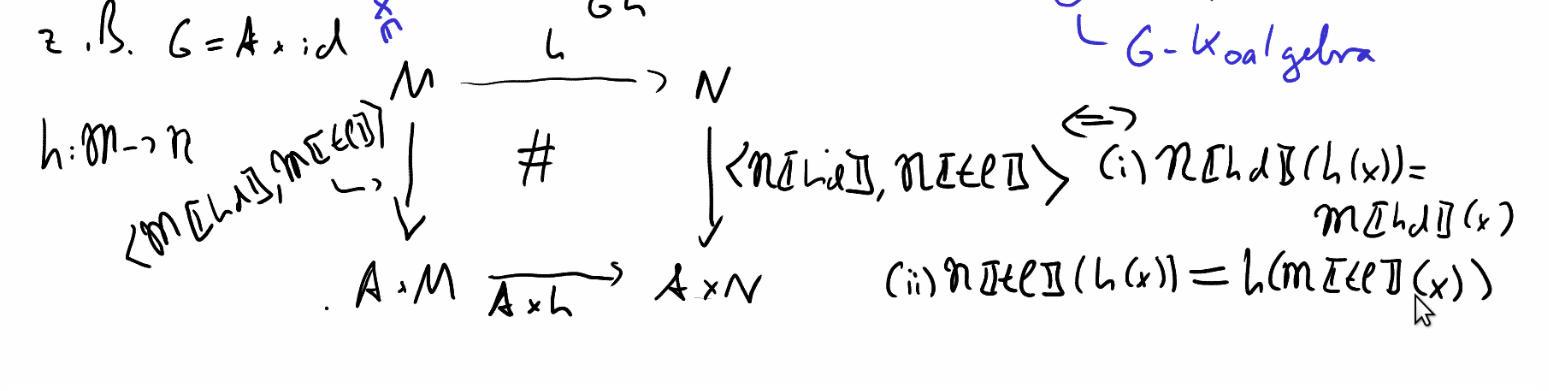
\includegraphics[width=256px]{images/G-KoalgebraBeispiel.png}\\
	Also das h bewahrt die heads.\\
	h ist mit der tail-funktion verträglich.\\
	\end{beispiel}
	\begin{definition} Eine G-Koalgebra $\mathfrak{N}$ ist final $\iff$ für jede G-Koalgebra $\mathfrak{M}$ existiert genau ein Morphismus $h:\mathfrak{M}\to\mathfrak{N}$\\
	\end{definition}
	\begin{satz} Die finale G-Koalgebra ist eindeutig modulo Isomorphismus (genauer: eindeutig bestimmter isomorphismus)
	\end{satz}
	\begin{beweis} Dual zur Eindeutigkeit initialer Algebren (zwischen zwei initialen Algebren gibt es einen homomorphismus, wenn beide initial sind,dann gibt die verkettung der morphismen die Ursprüngliche Algebra)
	\end{beweis}
	\begin{satz} Existenz der finalen Algebra\\
	Sei $G=A\times id$. $<hd,tl>:A^\omega\to A\times A^\omega$ ist finale G-Koalgebra.\\
	\end{satz}
	\begin{beweis}(anhand eines Beispiels für einfachere Notation\dots)\\
	Sei $\mathfrak{N}$ G-Koalgebra, schreibe $h_N = \mathfrak{N}\dbrack{hd}:N\to A$ $t_N = \mathfrak{N}\dbrack{tl}:N\to N$\\
	Setze $f:N\to A^\omega$ $f(x) = [a_0,a_1,\dots]$\\
	$a_0 = h_N(x)$,$a_1 = h_N(t_N(x))$ allg. $a_i = h_N(t^i_N(x))$\\
	Beh.: f ist der einzige Morphismus $\mathfrak{N}\to A^\omega$\\
	i) f ist ein Morphismus:\\
	$hd(f(x))\stackrel{!}{=}h_N(x)$\\
	$=h_N(t_N^0(x))$\\
	$tl(f(X)) = tl(a_0,a_1,\dots) = (a_1,\dots) =: (b_0,b_1,\dots)$\\
	$b_i=a_{i+1} = \underbrace{h_N (t_N^{i+1}(x))}_{``beobachtungskontext''} = hn(t_N^i(\underline{t_N(x)}))$\\
	also $(b_0,b_1,\dots) = f(t_N(x))$ d.h. f verträgt sich mit der Argumentation von tail\\
	wir iterieren mit $t_N$ und machen eine Observation mit $h_N$
	ii) Eindeutigkeit von f: Sei $g:\mathfrak{N}\to A^\omega$ Morphismus\\
	zZ $f=g$.\\
	Zeige $f(x)_i = g(x)_i$ wobei der index ``an der stelle i'' heißt. $\forall x\in N$\\
	durch Induktion über $i\in \mathbb{N}$:\\
	$i=0: g(x)_0 = hd(g(x)) \stackrel{morphismus}{=} h_N(x)=f(x) $\\
	$i\to i+1$: $g(x)_{i+1} \stackrel{indexversch}{=} (tl (g(x)))_i = \stackrel{morphismus}{=} g(t_N(x))_i \stackrel{IV}{=} f(t_N(x))_i = \dots =f(x)_{i+1}$ (Weil die Aussage für alle x gilt, und $t_N(x)$ ein x aus N ist)\\
	\end{beweis}
	\begin{definition} $h:N\to A, t:N\to N$\\
	definieren G-Koalgebra $\mathfrak{N}$, der eindeutige Morphismus $\mathfrak{N}\to A^\omega$ heißt
	 \[unfold\ h\ t\]
	unfold  h t ist definiert durch 2 Gleichungen:\\
	\begin{minted}{haskell}
		hd(unfold h t x) = h x
		tl(unfold h t x) = unfold h t (t x)
	\end{minted}
	\underline{Korekursive Definition}\\
	Man schreibt also für jeden Konstruktor eine funktion, die im korekursiven Fall beliebig oft eine Funktion auf den gegebenes Element x ausführt.\\
	\end{definition}
	\begin{beispiel} ones = 1,1,\dots\\
	\begin{minted}{haskell}
	ones = 1:ones
	\end{minted}
	\begin{minted}{Agda}
	hd ones = 1
	tl ones = 1
	\end{minted}
	blink x $(a_0,a_1,\dots) = (x,a_0,x,a_1,\dots)$\\
	\begin{minted}{Agda}
	hd (blink x s) = x
	tl (blink x s) = blink x ...???
	\end{minted}
	allgemeiner: blink: $2\times A\times A^\omega\to A^\omega$ wobei $2=\{0,1\}$\\
	Die 2 ist also ein ``merker'', bzw Extra Zustände in der Zustandsmaschine\\
	blink 0 x (a0,a1,...) = (x,a0,x,a1,...)\\
	blink 1 x (a0,a1,...) = (a0,x,a1,...)
	\begin{minted}{Agda}
	blink 0 = b0
	blink 1 = b1
	hd (b0 x s) = x
	tl (b0 x s) = b1 x s
	hd (b1 x s) = hd s
	tl (b1 x s) = b0 x (tl s)
	\end{minted}
	Das tail in b1 ist wichtig, weil wir das a0 auf a1 weiterschieben müssen\\
	\end{beispiel}
	\subsection{Koinduktion}
	$even:A^\omega \to A^\omega$\\
	even $(a_0, a_1, \dots)$ = $(a_0,a_2,a_4,\dots)$\\
	odd $(a_0, a_1, \dots)$ = $(a_1,a_3,a_5,\dots)$\\
	\begin{minted}{Agda}
	hd (even s) = hd s
	tl (even s) =even $tl $tl s
	hd (odd s) = hd $ tl s
	tl (odd s) = odd $tl $tl $ s
	\end{minted}
	Behauptung: odd $(b_0\ x\ s) = s$\\
	hd (odd $(b_0\ x\ s)$) = hd (tl $(b_0\ x \ s)$) = hd ($b_1$ x s) = hd s\\
	tl (odd $(b_0\ x\ s)$) = odd (tl tl $(b_0\ x\ s)$) = odd (tl ($b_1$ x s)) = odd ($b_0$ x (tl s)) $\stackrel{IV??????}{=}$ tl s\\
	Problem: wir reduzieren hier ``tl s$\to$ s'' aber hier wird ja nichts ``abgebaut'' die Streams werden also nicht kürzer!!!\\
	KOINDUKTION!! (``Circular Solver'')\\
	\begin{definition} Eine Relation $R\subseteq A^\omega\times A^\omega$ heißt Bisimulation, wenn für alle $(s,t)\in R$ gilt\\
	\begin{itemize}
		\item hd s = hd t
		\item (tl s) R (tl l)
	\end{itemize}
	\end{definition}
	\begin{satz} (Koinduktion). Wenn R eine Bisimulation ist, dann gilt $R\subseteq id$, d.h
	\[\forall s,t\in A^\omega (sRt)\implies s=t\]
	\end{satz}
	\begin{beweis} Sei $tl^n(s)Rtl^n(t)$. Per \underline{Induktion} über n folgt
	n=0 Annahme\\
	$n\to n+1$ per IV.
	\[\underbrace{tl(tl^n(s))}_{tl^{n+1}(s)}Rtl(tl^n(t))\]
	Es gilt also
	\[tl^i(s)Rtl^i(t)\ \text{ für alle }i\geq 0\]
	und damit
	\[hd(tl^i(s))=hd(tl^i(t))\text{ für alle } i\geq 0\]
	Damit folgt s=t\\
	Die Koinduktion ist also eigentlich nur eine Induktion über Destruktorkontexte!
	\end{beweis}
	\begin{beispiel} cont von oben\\
	Setze R=$\{(odd(b_0\ x\ s),s)|\forall s \in A^\omega\}$\\
	Zeige: R ist Bisimulation.\\
	Sei also $s\in A^\omega$\\
	i) hd($odd(b_0\ x\ s) $) = hd(s). Oben schon gezeigt.\\
	ii) tl($odd(b_0\ x\ s)$)R(tl s)\\
	linke Seite $=odd(b_0\ x (tl\ s))$, damit haben wir die Relation $\checkmark$
	\end{beispiel}
	\begin{beispiel} Zip-Funktion\\
	zip$:A^\omega\times A^\omega\to A^\omega$\\
	zip $(x_0,x_1,\dots)$ $(y_0,y_1,\dots)$ = $(x_0,y_0,x_1,y_1)$.\\
	hd(zip s t) = hd s.\\
	tl(zip s t)= zip t (tl s)\\
	(wir drehen also t und s um und entfernen den ersten Wert)\\
	Beh.: zip (even s) (odd s) = s.\\
	Setze R=$\{(zip(even\ s)(odd\ s),s)|\forall s\in A^\omega\}$\\
	zZ.: R ist Bisimulation. Sei also $s\in A^\omega$.\\
	i) hd (zip (even s) (odd s)) = hd (even s) = hd s $\checkmark$ wir haben die Relation\\
	ii) tl (zip (even s) (odd s))= zip (odd s) (tl (even s)) = zip (odd s) (even (tl (tl  (s)))) vs. tl s??????????\\
	also geht R nicht (R muss abgeschlossen sein, was es hier aber nicht ist)
	R' = $R\cup\{(zip (odd\ s) (even\ tl^2\ s), tl\ s)|\forall s\in A^\omega\}$\\
	R' ist Bisimulation:\\
	Paare in R schon bewiesen.\\
	neue Paare in R':\\
	i) hd(zip (odd s) (\dots)) = hd (odd s) = hd (tl s)$\checkmark$\\
	ii) tl(zip (odd s) (even $tl^2$ s) ) = zip (even ($tl^2$ s)) $\underbrace{(tl (odd s))}_{odd(\underline{tl^2\ s})}$ R'(tl(tl s))\checkmark.\\
	Entspricht also verstärkung des Induktionszieles.\\
	\end{beispiel}
	\subsection{kodatentypen mit mehreren Nachfolgeoperationen}
	\begin{minted}{agda}
	codata Tree where
	 out:   Tree -> A
	 left:  Tree -> Tree
	 right: Tree -> Tree
	\end{minted}
	definiert die finale G-Koalgebra für $G=A\times id\times id$\\
	Diese besteht aus unendlichen binären Bäumen mit in A beschrifteten Knoten.\\
	$mirror:Tree\to Tree$ Korekursiv definiert durch\\
	\begin{minted}{agda}
	out (mirror t) = out t
	left (mirror t) = mirror (right t)
	right (mirror t) = mirror (left t)
	\end{minted}
	$R\subseteq Tree\times Tree$ ist Bisimulation $\iff$ $\forall(s,t)\in R$\\
	i) out s = out t\\
	ii) (right s) R (right t)\\
	iii) (left s) R (left t)\\
	(analog wie bei Streams, nur mit 2 ``tail'' funktionen)\\
	\begin{beispiel} Beh.: mirror (mirror t) = t.\\
	Setze R = $\{(mirror(mirror\ t),t)|\forall t\in Tree\}$ (eig. Semantikklammern um Tree, wird hier ``wegvereinfacht'')\\
	Zeige: R ist eine Bisimulation.\\
	Sei also $t\in Tree$\\
	i) out (mirror (mirror t)) = out(mirror t) = out t.$\checkmark$\\
	ii) left(mirror(mirror t)) = mirror (right(mirror t)) = mirror (mirror (left t)) R( left t)\\
	weil oben in R als beliebiges t auch (left t) gewählt werden kann.\\
	iii) analog \\
	right(mirror(mirror t)) = mirror (left(mirror t)) = mirror (mirror(right t)) R (right t)\\
	\end{beispiel}
	\underline{Nebenbemerkung}: Es gibt auch Abbrechende Streams von Typ $1+A\times X$ (gleiche System von Listen). Hier gibt es 2 optionen: Wir kriegen einen neuen Stream bei tail, den head, oder ein Ende. (vgl Skript 4.8)\\
	\section{Polymorphie}
	polymorphe Funktionen: anwendbar auf Argumente verschiedenen Typs.\\
	ad-hoc-Polymorphie: +\\
	parametrische Polymorphie\\
	swap (x,y) = (y,x)\\
	swap:$a\times b\to b\times a$\\
	d.h. Das genau gleich stückchen code bekommt verschiedene typen (im gegensatz zu ad-hoc, wo im einen fall int, im anderen float addition ausgewählt wird).\\
	concat: List a$\to$ List a$\to$ List a.\\
	ist auch parametrisch polymorph.\\
	\subsection{System F}
	silly::Bool\\
	silly=($\lambda xy.x$)(id True)(id 42)\\
	Im einfach getypten Lambda Kalkül kann man das nicht typen: $id:Bool\to Bool$ und gleichzeitig $id:Int\to Int$!\\
	Typen in System F:\\
	\[\alpha,\beta::=a|\alpha\to\beta |\forall a.\alpha\ \ (a\in V)\]
	z.B.: $id:\lambda x.x:\forall a.a\to a$\\
	Typregeln: $\lambda\to$ plus\\
	\AxiomC{$a\notin FV(\Gamma)$}
	\AxiomC{$\Gamma\vdash s:\alpha$}
	\LeftLabel{$(\forall_i)$}
	\BinaryInfC{$\Gamma\vdash s:\forall a.\alpha $}
	\DisplayProof\\
	\AxiomC{$\Gamma\vdash s:\forall a.\alpha$}
	\LeftLabel{$(\forall_e)$}
	\UnaryInfC{$\Gamma\vdash s:(\alpha[\beta/a])$}
	\DisplayProof\\
	\begin{beispiel}.\\
	\AxiomC{}
	\RightLabel{NICHT $x:a|x:\forall a.a$, das a ist im Kontext}
	\LeftLabel{(Ax)}
	\UnaryInfC{$x:a\vdash x:a$}
	\LeftLabel{($\to_i$)}
	\UnaryInfC{$\vdash \lambda x.x: a\to a$}
	\LeftLabel{$\forall i$}
	\UnaryInfC{$\vdash \lambda x.x: \forall a. a\to a$}
	\DisplayProof\\
	\end{beispiel}
	\subsection{Church-Kodierung in System F}
	$\mathbb{N}$ ist initiale $\Sigma_{Nat}$-Algebra $\Sigma_{Nat} =\{0/0,s/1\}$\\
	\begin{itemize}
		\item $\mathbb{N}:=\forall a.(a\to a)\to a\to a$
		\item $0:\mathbb{N}$\\
		 $0=\lambda fx.x$ hat den typ von oben\\
		\item $s:\mathbb{N}\to \mathbb{N}$\\
		$s\ = \underbrace{\lambda\ n}_{wir\ kriegen\ ein\ \mathbb{N}}.\lambda\ f\ x.f(n\ f\ x)$\\
		Haskell mit GHC: Higher-Rank-polymorphism
		\item fold:$\forall a.(a\to a)\to a\to \mathbb{N}\to a$\\
		fold = $\lambda f\ x\ n.n\ f\ x$ also n mal f auf x anwenden.
	\end{itemize}
	Paare:
	\begin{itemize}
		\item $(a\times b):=\forall r\underbrace{(a\to b\to r)}_{f}\to r$ (sprich ich kann ein paar aus ab zu einem r machen, effektiv uncurry)
		\item pair:$\forall ab: a\to b\to( a\times b)$\\
		pair = $\lambda x y.\lambda f.f\ x\ y$
		\item fst:$\forall ab. (a\times b)\to a$
		fst = $\lambda p.p\underbrace{(\lambda\ x\ y.x)}_{das\ ist\ das\ zugeordnete\ f}$ wir haben also eine pick-funktion, die das erste paarelement gibt, das zweite ignoriert
	\end{itemize}
	Summen:
	\begin{itemize}
	 \item (a+b):$\forall r.\underbrace{(a\to r)}_{f}\to \underbrace{(b\to r)}_{g}\to r$
	 \item inl:$\forall ab.a\to (a+b)$\\
	 inl = $\lambda x.\lambda f\ g. f\ x$\\
	 \item case: $\forall abs. (a\to s)\to (b\to s)\to (a+b)\to s$\\
	 case = $\lambda\ f\ g\ z.z\ f\ g$
	\end{itemize}
	Listen:
	\begin{itemize}
		\item List a:$\forall r.r\to (a\to r\to r)\to r$\\
		Nil: $\forall a. List\ a$\\
		Nil = $\lambda u\ f. u$\\
		Cons: $\forall a. a\to List\ a\to List\ a$\\
		Cons = $\lambda u\ f. \lambda v\ g.g\ u(f\ v\ g)$
	\end{itemize}
	Herleitung der Typisierung von suc\\
	\AxiomC{ist typ von $\mathbb{N}$}
	\LeftLabel{(AX)}
	\UnaryInfC{$\Gamma\vdash \forall a.(a\to a)\to a\to a$}
	\LeftLabel{$(\forall_e)$}
	\UnaryInfC{$\Gamma\vdash n:(a\to a)\to a\to a$}
	\UnaryInfC{$\vdots$}
	\LeftLabel{für f und x typen aus kontext}
	\UnaryInfC{$\Gamma\vdash n\ f\ x:a$}
	\AxiomC{}
	\LeftLabel{(Ax)}
	\UnaryInfC{$\Gamma\vdash f:a\to a$}
	\LeftLabel{$\to_e$}
	\BinaryInfC{$\underbrace{n:\mathbb{N};f:a\to a;x:a}_{\Gamma}\vdash f\ (n\ f\ x):a$}
	\LeftLabel{$2\times\to_i$}
	\UnaryInfC{$n:\mathbb{N}\vdash \lambda\ f\ x.\ f\ (n\ f\ x):(a\to a)\to a\to a$}
	\LeftLabel{$\forall_i$}
	\RightLabel{zum auflösen von $\mathbb{N}$}
	\UnaryInfC{$n:\mathbb{N}\vdash \lambda\ f\ x.\ f\ (n\ f\ x):\mathbb{N}$}
	\LeftLabel{($\to_i$)}
	\UnaryInfC{$\vdash \lambda\ n\ f\ x.\ f\ (n\ f\ x):\mathbb{N}\to\mathbb{N}$}
	\DisplayProof\\
	\newpage
	\begin{satz} Wells 1994: Typcheck in System F ist untentscheidbar!\\
	Jede arithmetik 2. Stufe definierbar totale berechenbare Funktion ist in System F typisierbar!! (Reicht um die Reellen Zahlen zu typisieren!)
	\end{satz}
	\begin{satz} (Normalisierend, Girard) System F ist SN, wenn $\Gamma\vdash s:\alpha$ in $\lambda 2$ dann ist s stark normalisierend (also System F nicht Turingmächtig)
	\end{satz}
	Trotzdem in System F ist definierbar
	\begin{itemize}
		\item alle primitiv rek. Funktionen
		\item Ackermann
		\item Compiler, aber nicht Interpreter
	\end{itemize}
	\subsection{ML-Polymorphie}
	Einschränkungen:\\
	1) $\forall$ nur top-level.\\
	2) Mehrfachinstanziierung nur per let!\\
	$(\lambda f.ff)\underbrace{(\lambda x.x)}_{id}$\\
	ist let $\underbrace{f=\lambda x.x}_{\forall a.a\to a}$ in f f.\\
	Typen
	\[\alpha,\beta::= a|\alpha\to\beta\]
	Typschemata gebe durch die nicht rekursive Grammatik
	\[S::= \forall a_1,\dots,a_k.\alpha\text{ mit } (k\geq 0)\]
	Terme
	\[t,s::=x|ts|\lambda x.t|let\ x=s\ in\ t\]
	in System F sind variablen, die nicht verwendet werden implizit alquantifiziert.\\
	Wir definieren eine Closure
	\[Cl(\Gamma,\alpha)=\forall a_1,\dots,a_k.\alpha\ \text{mit }\ \{a_1,\dots,a_k\}= FV(\alpha)\setminus FV(\Gamma)\]
	Typschemata in $\Gamma$. Also alle typen sind Tyschemata, aber nicht alle Typschemata sind typen!\\
	Die Tyschemata kommen nur im Kontext vor, man kann keine Funktion selbst polymorph machen, nur sagen, dass eine Poylmorphes ``ding'' im kontext steht.\\
	Typregeln $(\to_i),(\to_e)$ gleich\\
	\AxiomC{}
	\RightLabel{$(x:\forall a_1,\dots, a_k.\alpha\in\Gamma)$}
	\LeftLabel{$\forall_e$}
	\UnaryInfC{$\Gamma\vdash x:\alpha[\beta_1/a_1,\dots,\beta_k/a_k]$}
	\DisplayProof\\
	Effektiv wird hier also $\forall_e$ immer kombiniert mit einer Ax Regel ausgeführt. Dies liegt daran, dass wir Termen kein Typschema, sondern nur Typen zuweisen können)
	\\
	\AxiomC{$\Gamma[x\mapsto Cl(\Gamma,\alpha)]\vdash t:\beta$}
	\AxiomC{$\Gamma\vdash s:\alpha$}
	\RightLabel{$(x:\forall a_1,\dots, a_k.\alpha\in\Gamma)$}
	\LeftLabel{let}
	\BinaryInfC{$\Gamma\vdash$ let x=s in t $:\beta$}
	\DisplayProof\\
	Dies ersetzt die $\forall_i$ wir setzen also alle noch nicht vom Kontext festgelegten werte frei im Let. Wir lassen also keine funktionen mehr von polymorphen funktionen abhängen, stattdessen benutzen wir das let und passen das Typschema an.\\
	Kontexte bestehen aus $\Gamma =\{x_1:S_1,\dots,x_n:S_n\}$ also aus Typschemata.\\
	\begin{beispiel}.\\
	\AxiomC{z.B. $\gamma=a\to a$}
	\LeftLabel{$(\forall_e)$}
	\UnaryInfC{$id:\forall a.a\to a\vdash id:\gamma$}
	\AxiomC{z.B. $\beta=a\to a$}
	\LeftLabel{$(\forall_e)$}
	\UnaryInfC{$id:\forall a.a\to a\vdash id:\gamma\to\beta$}
	\LeftLabel{$\to_e$}
	\BinaryInfC{$id:\forall a.a\to a\vdash id\ id:\beta$}
	\RightLabel{implizite allquantifizierung von a explizit}
	\AxiomC{$\hdots$}
	\LeftLabel{(herleitung $\lambda\to$)}
	\UnaryInfC{$\vdash \lambda x.x$}
	\LeftLabel{(let)}
	\BinaryInfC{$\vdash$let id = $\lambda x.x$ in id id:$\beta$}
	\DisplayProof\\
	\end{beispiel}
	Wenn wir den Hindley-Millner algorithmus generalisieren wollen, brauchen wir die Typinversionsregeln.\\
	Diese gelten aber in System F nicht (das macht genau die Entscheidbarkeit kaputt)\\
	\begin{satz} Inversionslemma: Applikation,$\lambda$ wie für $\lambda\to$\\
	- Variablen: $\Gamma\vdash x:\alpha\iff \Gamma(x)=\forall a_1,\dots, a_k.\beta$\\
	$\alpha$ hat die Form $\alpha =\beta[\gamma_1/\alpha_1,\dots,\gamma_k/\alpha_k]$\\
	- let: $\Gamma\vdash let\ x= s$ in t$:\beta$ $\iff\Gamma\vdash s:\alpha, \Gamma[x\mapsto Cl(\Gamma,\alpha)]\vdash t:\beta$\\
	\end{satz}
	Recall: $PT(\Gamma,t,\alpha)$ Gleichunssystem\\
	\underline{Invariante}: $\sigma$ löst $\Gamma\vdash t:\alpha$ $\iff \sigma$ erweitert zu Unifikator von $PT(\Gamma,t,\alpha)$\\
	\begin{definition} von $PT(\Gamma,t,\alpha)$ per Rekursion über t.\\
	Klauseln für Applikation, $\lambda$ wie in $\lambda\to$\\
	$PT(\Gamma,x,\alpha)=\{\beta[a_1'/a_1,\dots a_k'/a_k] \doteq \alpha\}$ für $\Gamma(x)=\forall a_1,\dots,a_k.\beta$ sprich wir müssen verlangen, dass die allquantifizierten variablen von $\beta$ frisch sind\\
	$PT(\Gamma,let\ x=s\ in\ t;\alpha)=PT(\Gamma\sigma[x\mapsto Cl(\Gamma\sigma,\sigma(a))];t;\alpha\sigma)$\\
	$\sigma = $mgu($PT(\Gamma,s,a)$ (a frisch)) wir machen also Typinferenz für s und substituieren passend.\\
	\end{definition}
	\begin{beispiel} $PT((); let\ id\ = \lambda x.x\ in \ id\ id; a)$\\
	zuerst das let auflösen, dafür PT von $\lambda x.x$ bestimmen\\
	$mgu(PT(();\lambda x.x; b))$; $\sigma(b)=c\to c$\\
	jetzt das Closure einsetzen für let\\
	$PT(\underbrace{id:\forall c.c\to c}_{\Gamma}; id\ id; a)$\\
	$=PT(\Gamma; id; d\to a)\cup PT(\Gamma, id; d)$\\
	$=\{c\to c\doteq d\to a\}\cup \{\underbrace{e\to e}_{global\ frisch} \doteq d\}$\\
	der mgu ist also $\color{red} a\doteq e\to e$
	\end{beispiel}
	\begin{beweis} Korrektheit Invariante\\
	Variablen: wenig neues (wir machen jetzt nur ein instanziierung, die vom unifikationsalgorithmus sowieso gemacht wird)\\
	\begin{definition} Für $S=\forall a_1,\dots,a_k.\alpha$\\
	Inst(S) =$\{\alpha[\beta_1/a_1,\dots,\beta_k/a_k|\beta_1,\dots, \beta_k\text{ Typen}\}$\\
	S allgemeiner als $S'$ $\iff$ Inst(S')$\subset Inst(S)$\\
	\end{definition}
	\begin{lemma} Für $S=\forall a_1,\dots, a_k.\alpha, S'=\forall b_1,\dots, b_m.\beta$ sind äquivalent:\\
	i)  S allgemeiner als S'\\
	ii) $\beta\in Inst(S)$ UND $b_1\dots b_m\notin FV(\alpha)$\\
	Das Liefert u.U. aber ein Problem $S=\forall a.a\to b$ $S' = \forall b.b\to b$ hier ist S nicht allgemeiner als S', obwohl man einfach a=b wählen kann\\
	\begin{beweis} (nur ii nach i, andere Richtung geht, brauchen wir aber nicht)\\
	Sei $\beta=\alpha[\gamma_1/a_1,\dots,\gamma_k/a_k]$, $\sigma = [\delta_1/b_1,\dots,\delta_m/b_m]$ (d.h. $\beta\sigma\in$ Inst(S'))\\
	zZ $\beta\sigma\in Inst(S)$\\
	Nach Annahme\\
	$\beta\sigma =\alpha[\gamma_1\sigma/a_1,\dots \gamma_k\sigma/a_k]\in Inst(S)$
	\end{beweis}
	\end{lemma}
	Damit folgt
	\begin{lemma} $CL(\Gamma,\alpha)\sigma$ allgemeiner als $CL(\Gamma\sigma,\alpha\sigma)$\\
	\begin{beweis} i) Klar $\checkmark$\\
	ii): Quantifizierte Variablen rechts: $FV(\alpha\sigma)\setminus FV(\Gamma\sigma)$\\
	d.h. $b\in FV(CL(\Gamma,\alpha)\sigma)\implies b\in FV(\sigma(a))$ für ein $a\in FV(CL(\Gamma,\alpha))\subseteq FV(\Gamma)$\\
	$\implies b\in FV(\Gamma\sigma)$,\\
	also b rechts nicht quantifiziert.\\
	\end{beweis}
	\end{lemma}
	\begin{lemma} Abschwächung:\\
	S allgemeiner als S', $\Gamma,x:S'\vdash t:\alpha$\\
	$\implies \Gamma,x:S\vdash t:a\alpha$, Klar.
	\end{lemma}
	Invariante für let:\\
	(nur $\implies$ weil $\impliedby$ direkt folgt, weil wir mehr unifizieren, als wir brauchen, also auch insbesondere unser let)\\
	Sei $\Gamma\sigma\vdash let\ x= s\ in\ t:\alpha\sigma$.\\
	Per Inversionslemma es existiert $\beta$ mit $\Gamma\sigma\vdash s:\beta,\Gamma\sigma,x:CL(\Gamma\sigma,\beta)\vdash t:\alpha\sigma$\\
	$\stackrel{IV}{\implies}\sigma$ erweiterbar zu $\sigma'\in Unif(PT(\Gamma\sigma;s;b))$ mit $\sigma'(b)=\beta$\\
	$\tau:=mgu(PT(\Gamma\sigma;s;b));$ GLOIN: o.E.$\tau\sigma'=\sigma'$\\
	zZ: $\sigma'$ erweitert zu Unifikator von $PT(\Gamma\tau, x:CL(\Gamma\tau,\tau(b)),t,\alpha\tau)$\\
	I.V.: reicht $\Gamma\tau\sigma',x:CL(\Gamma\tau,\tau(b))\sigma'\vdash t:\alpha\tau\sigma'$\\
	$\iff \Gamma\sigma,x:CL(\Gamma\tau,\tau(b))\sigma'\vdash t:\alpha\sigma$\\
	$\iff \Gamma\sigma,x:CL(\Gamma\sigma,\sigma(b))\vdash t:\alpha\sigma$\\
	Man kann das $\sigma'$ reinziehen (das geht per lemma, weil wir sogar weniger allgemein auf der rechten seite werden)
	\end{beweis}
	\section{Automatentheorie}
	(Gerade Rechtzeitig\dots)\\
	\subsection{Sprachen als Kodaten}
	Recall: DFA A = $(Q,\Sigma,\delta, s, F)$\\
	\begin{itemize}
		\item Q (endliche) Menge von Zuständen
		\item $\Sigma$ Alphabet (endlich)
		\item $\delta : Q\times (\Sigma\cup\{\epsilon\})\to Q$
		\item Anfangszustand $s\in Q$
		\item Menge $F\subseteq Q$ von akzeptierenden/finalen Zuständen
	\end{itemize}
	\begin{definition} $\delta(q,w)$ für $w\in\Sigma^*$ induktiv
	\[\delta(q,\epsilon)=q\]
	\[\delta(q,wa)=\delta(\delta(q,w),a)\]
	(von hinten erweitern ist einfacher, wir schalten Buchstabe für Buchstabe durch das Wort)\\
	Von A akzeptierte Sprache\\
	\[L(A) =\{ w\in\Sigma^*|\delta(s,w)\in F\}\]
	(Praxisrelevanz: Programme sind meistens automaten (u.u. endlich), d.h. es wurden schon pinautomaten geknackt, indem man automatisch den automatenuntersucht hat)\\
	Schreibe $\delta : Q \to (\Sigma\to Q)$, $F:Q\to 2$\\
	wir haben also $<F,\delta>:Q\to \underbrace{2\times \overbrace{(\Sigma\to Q)}^{\cong Q\times \dots\times Q,|\Sigma|\ mal}}_{GQ}$ wir haben also eine (rekursive) G-Koalgebra.\\
	bzw. Es fehlt noch der intialzustand, wir nennen diese Vorstufe eine (deterministisches) Transitionssystem $A_0$
	\begin{minted}{haskell}
		codata Lang Sigma where
			acc : Lang Sigma -> Bool
			der : Lang Sigma -> (Sigma -> Lang Sigma)
			-- accept/derivation
	\end{minted}
	\end{definition}
	der sind eigentlich viele nachfolgeoperationen: Eine pro $\Sigma$.\\
	finale Koalgebra:
	- unendliche $\Sigma$-verzweigenden Bäumen\\
	- Knoten in 2 gelabled (also $T,\bot$)\\
	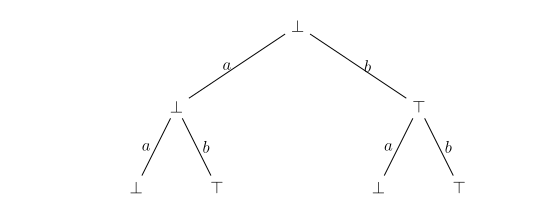
\includegraphics[width=256px]{images/AutomatenAlgebra.png}\\
	Es ändert sich eigentlich nur, welche Lables in jedem schritt gesetzt werden (links bleibt a, rechts b)\\
	Allgemein kann somit der Baum mit Worten indiziert werden. Der Baum hier entspricht also einer Teilmenge aus $\Sigma^*$ ist also eine Sprache.\\
	\[F(L)\epsilon=T\iff \epsilon\in L\]
	\[\delta\ L\ a =\{u\in\Sigma|au\in L\} = L_a\]
	wobei $L_a$ Ableitung von L nach a ist. (wir schalten mit $\delta$ durch den Ableitungsbaum)\\
	$\Lambda = P(\Sigma^*)$ bezeichnet sowohl die Menge aller Sprachen, als auch die finale G-Koalgebra\\
	G-Koalgebramorphismen:\\
	Sei A, B automaten und f eine funktion von $Q_A\to Q_B$
	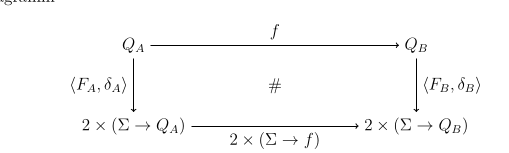
\includegraphics[width=256px]{images/AutomatenHomomorphismus.png}\\
	(b,g) $\mapsto$ ($b, f\circ g$)\\
	links: $F_B(f(q)) = F_A(q)$ d.h. $f(q)$ final $\iff$ q final.\\
	Also wenn wir im Urbild fertig sind, dann muss auch das Bild fertig sein.\\
	rechts: $\delta_B(f(q)(a)) = f(\delta_A(q)(a))$ wir können also eine Transition in $Q_A$ machen, und den fortschritt in $Q_B$ bringen.\\
	\begin{satz} Sei $A_0 = (Q,\Sigma,\delta_A,F_A)$ Transitionssysteme.\\
	Der eindeutige G-Koalgebramorphismus $f:A_0\to \Lambda$ ist
	\[f:Q\to\Lambda\]
	\[q\mapsto L(A_0,q) = \{w|F(\delta(q)(w)) = T\}\]
	(in anderen worten: f bildet von automaten auf die akzeptierende Sprache ab)
	\end{satz}
	\begin{beweis} Reicht: f ist Morphismus\\
	Finalität wird bewahrt: q final $\iff$ $\epsilon\in L(A_0,q)\iff L(A_0,q)$ final in $\Lambda$\\
	Transitionen: zZ $\overbrace{f(\delta_A(q)(a))}^{L(A_0,\delta_A(q)(a)}=\delta_\Lambda (f(q))(a) = L(A_0,q)a$\\
	$u\in L(A_0, \delta_A(q)(a))\iff F_A(\underbrace{\delta_A(\delta_A(q)(a))(u)}_{=\delta_A(q)(au)}) = T \iff au\in L(A_0,q)\iff u\in L(A_0,q)_a$
	\end{beweis}
	\begin{korrolar}\label{KorrolarSprache} 1) $L\in\Lambda\implies L(\Lambda, L) = L$\\
	 ($\Lambda$ ist ein Automat, L eine Sprache in diesem (undendlichen Automat))\\
	 2) $f:A_0\to B_0$ Morphismus von Transitionssystemen $\implies L(A_0,q)= L(B_0,f(q))$
	 \end{korrolar}
	 \begin{beweis}.\\
	 1)\\
	 
\includegraphics[width=128px]{images/LausLambda.png}
	 2)\\
	 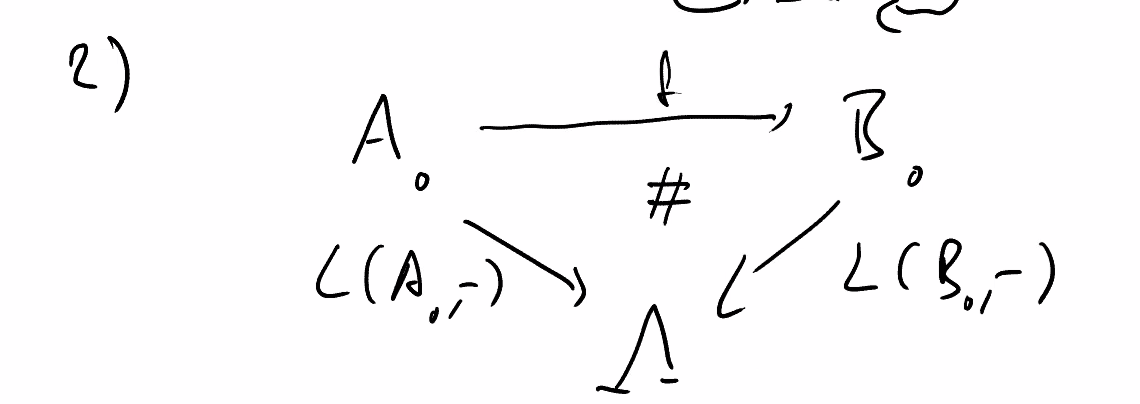
\includegraphics[width=256px]{images/Kommutation.png}
	 \end{beweis}
	 \subsection{Minimierung}
	 Wir haben 2 grobe Fälle: Zustände können equivalent sein, oder Nutzlos (unerreichbar)
	 \begin{definition} Sei $A_0$ Transitionssystem $q\in Q_0$
	 \[<q> =\{\delta(q)(w) | w\in\Sigma^*\}\]
	 Das sind alle von q aus erreichbaren Zustände. Wir nennen dies das von q erzeugte Untertransitionssystem.\\
	 \end{definition}
	 Es ist Tatsächlich ein Untertransitionssystem, weil $q'\in <q>$ final $\iff$ $q'$ final in $A_0$\\
	 $\underbrace{\delta_{<q>}(q')(a)}_{\delta(q)(w)}=\underbrace{\delta_{A_0}(q')(a)}_{\delta(q)(wa)\in <\delta>}$\\
	 somit unter Transition abgeschlossen.
	 \begin{lemma}\label{einbettung} Die Einbettung $<q>\hookrightarrow A_0$ Morphismus, sodass die Behauptungen aus dem Korrolar \ref{KorrolarSprache}
	 (die Eigentliche Einbettung ist ein Noop von $q\to q$, zeigt nur eine Teilmengeneigenschaft auf der Algebra)
	 \end{lemma}
	 \begin{lemma} .\\
	 \[f:A_0\to B_0\]
	 Morphismus $\implies$
	 \[f:<q>\to <f(q)>\]
	 Morphismus, surjektiv\\
	 (aus surjektiv folgt insbesondere $|<f(q)>|\leq |<q>|$)
	 \end{lemma}
	 \begin{beweis}.\\
	 $\{\delta_{A_0}(q)(w)|w\in\Sigma^*\}$ $\{\delta_{B_0}(q)(w)|w\in\Sigma^*\}$\\
	 f kommutiert $f(\delta_{A_0}(q)(w))=\delta_{B_0}(f(q))(w)$\\
	 Damit sind beide Behauptungen gezeigt.
	 \end{beweis}
	 \begin{lemma} $L(<q>,q) = L(A_0,q)$ folgt aus \ref{einbettung}
	 \end{lemma}
	 z.B. $f = L(A_0,-)$ ist ein Morphismus:
	 \[|<L(A_0,q)>| \leq |<q>| \leq |A_0|\]
	 d.h. $L(A)=L \implies |<L>|\leq |A|\implies L(\Lambda, L) = L(<L>,L) =L $ $(<L>,L)$ ist minimaler Automat für L. (besteht aus allen von m aus erreichbaren Sprachen im Transitionssystem)
	 \begin{satz} L regulär $\iff$ $<L>$ endlich.
	 \end{satz}
	 Recall:  R Äquivalent auf X $\implies X/R =\{[x]_R|x\in X\} = \{y|xRy\}$\\
	 $|x/R| =$ Index von R.\\
	 $f: X\to Y$\\
	 $Ker (f) = \{(x,y)| f(x) = f(y)\}$ ist eine Äquivalenz (Das ist eine generalisierung von Ker aus linAlg $f(x)=f(y)\iff f(x)-f(y)=0\iff \underbrace{f(x-y)}_{linear} =0\iff x-y\in Ker(f)$)\\
	 \[h: X/(Ker(f))\to f[X] =\{f(x) | x\in X\}\]
	 \[[x]_{Kerf} \mapsto f(x) \text{  bijektiv}\]
	 h wohldefiniert: x(Kerf)y $\implies f(y)=f(x)$ DAS HIER IST WOHLDEFINIERT (die Abbildung ist von representanten unabhängig, NICHTS anderes)\\
	 also index von Kerf = $|f[x]|$
	 \[<L> = \{L_u | u\in \Sigma^*\} = d[\Sigma^*],\]
	 mit $d(u) = L_u\implies <L>$ endlich $\iff \Sigma^*/(Kerd)$ endlich.\\
	 $\sim_L := Kerd$
	 \[v\sim_L w\iff L_v = L_w \iff \forall u\in \Sigma^* (u\in L_v \iff u\in L_w)\]
	 \[\forall u\in \Sigma^* (vu\in L\iff wu\in L)\]
	 \begin{satz} von Myhill/Nerode: L regulär $\iff \sim_L$ hat endlichen Index.\end{satz}
	 Bisimulation auf $\Lambda$: $R\subseteq \Lambda\times\Lambda$ Bisimulation $\iff$ L R K $\implies$\\
	 1) $\sigma\in L\iff \sigma\in K$ (also $F(L)=T\iff F(k)=T$)\\
	 2) $\forall a\in \Sigma(\underbrace{\delta(L)(a))}_{L_a} R \underbrace{\delta(K)(a)}_{K_a})$\\
	 allgemeiner: $A_0 = (Q,\Sigma,\delta,F)$ Transitionssystem\\
	 $R\subseteq Q\times Q$ Bisimulation $\iff \{(L(A_0,q),L(A_0,r))| (q,r)\in R\}$ Bisimulation auf $\Lambda$ (sprich, wenn die Sprache von q und die Sprache von r über A in Relation stehen)\\
	 d.h. $(q,r)\in R\implies$\\
	 1) $F(q)=F(r)$
	 2) $\forall a\in\Sigma(\delta(q)(a)R\delta(r)(a))$\\
	 q,r \underline{bisimilar} (ist die größte Bisimulation zwischen q und r) $\iff \exists R$ Bisimulation (qRr)\\
	 q,r bisimlar $\implies$ $L(A_0,q)=L(A_0,r)$\\
	 ALGORITHMUS (Minimiere DFA A=$(Q,\Sigma,\delta,s,F)$)
	 var $R\subseteq Q\times Q$
	\begin{itemize}
	 \item 1. Entferne nicht erreichbare Zustände aus Q (Tiefensuche, merke gefunde Zustände, sobald ein Zustand doppelt, kann dieser Teilbaum abgebrochen werden)
	 \item 2. Initialisiere $R=\{(q,r)\in Q\times Q| q\in F\iff r\in F\}$ (R hat erstmal 2 Äquivalienzklassen: final/nichtfinal, wir nähern die größte bisimulation von oben her an; bisimilar 1 gilt)\\
	 \item 3. Pick $(q,r)\in R, a\in \Sigma$ mit
	 \[(\delta(q)(a),\delta(r)(a))\notin R\]
	 if not found goto 4
	 else $R:= R\setminus \{\overbrace{(r,q),(q,r)}^{symmetrie}\}$ goto 3
	 \item 4. $Q:=Q/R, f:=F/R, \delta([q]_R)(a)=[\delta(q)(a)]_R$ wir reduzieren also den automaten auf die Äquivalenzklassen
	\end{itemize}
	\begin{satz} Nach Schritt 4 ist	A minimal (nach Quotientierung durch R)
	\end{satz}
	\begin{beweis} Reich $q,r$ bisimilar (im Input) $\iff qRr$ in Schritt 4.\\
	``$\impliedby$'' per 2,3 ist R am ende eine Bisimulation. (in 2. werden alle finalen und nichtfinalen getrennt, in 3. werden alle nicht äquivalenten zustände getrennt)\\
	``$\implies$'' Entfernte Paare sind nicht bisimilar (Invariante des Algorithmus)
	\end{beweis}
	\begin{beispiel}.\\
	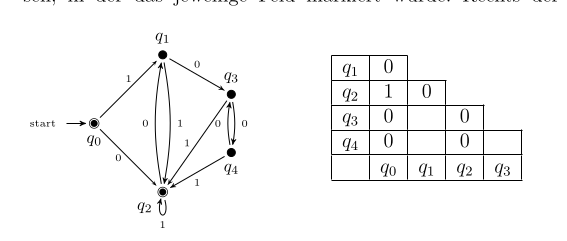
\includegraphics{images/MinimierungBsp.png}\\
	Dreieckig, weil symmetrisch, auch die diagonale kann weggelassen werden (Äq-Relation ist trivial Reflexiv)
	Die zahl ist die Optimierungsrunde, in der die Zustände rausfliegen.\\
	Runde Null lässt Zustände mit unterschiedlicher finalität rausfliegen.\\
	Erste runde z.B. $q_2$ hat 1 nachfolger $q_2$ und $q_0$ hat 1 nachfolger $q_1$. $q_1$  und $q_2$ sind nicht in relation (per schritt 0) fliegt raus.\\
	aber z.B. $q_3,q_4$ haben beide als 1 nachfolger $q_2$ und 0 nachfolger $q_3$ und $q_4$, die beide in Relation stehen (wir checken ja gerade das, deshalb müssen sie noch drin sein) \\
	Die leeren stellen sind die in relation stehenden zustände\\
	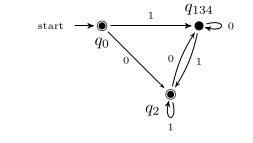
\includegraphics{images/MinimalerAutomat.png}
	die Übergänge können einfach durch einen der Nachfolger bestimmt werden (welcher ist egal, die sind ja äquivalent)
	\end{beispiel}
	\section{Bonus: SN von System F}
	Idee: zu Typ $\alpha$ definiere
	\[\dbrack{\alpha}_{\xi} \subseteq SN = \{t\in \Lambda|t\ SN\}\]
	mit $\xi: V\to SAT$
	\[SAT = \{A\subseteq SN| A\ saturiert\}\]
	\[A\to B = \{t\in\Lambda| \forall s\in A.\ ts\in B\}\]
	mit $A,B\subseteq \Lambda$\\
	Rekursiv 3 Fälle:
	\[\dbrack{\alpha}_{\xi} =\xi(\alpha)\]
	\[\dbrack{\alpha\to\beta}_{\xi} = \dbrack{\alpha}\to\dbrack{\beta}\]
	\[\dbrack{\forall a.\alpha}_{\xi} = \bigcap_{A\in SAT}\dbrack{\alpha}_{\xi[a\mapsto A]}\]
	(der letzte punkt ist ein Durchschnittstyp: das macht das ding untentscheidbar)
	\begin{lemma} Substitutionslemma (noch eins)\\
	\[\dbrack{\alpha[\beta/a]}_\xi = \dbrack{\alpha}_{\xi[a\mapsto\dbrack{\beta}_\xi]}\]
	Beweis: Induktion über $\alpha$
	\end{lemma}
	\begin{definition} $A\subseteq SN$  \underline{saturiert} $\iff$\\
	i) $xt_1\dots t_n\in A$ ($x\in V;t_1,\dots,t_n\in SN;n\geq 0$)\\
	ii) $t[s/x] u_1\dots u_n\in A\implies $\\
	$(\lambda x.t)su_1\dots u_n\in A (s, \in SN)$ (wir müssen explizit s SN annehmen, weil x u.U. nicht in t existiert: es viele also in der prämisse weg. Die konklusion ist dann aber abhängig von reduktionsreihenfolge, also nicht mehr SN!)\\
	\end{definition}
	\begin{lemma} Saturiertheitslemma\\
	a) $SN\in SAT$\\
	b) $\dbrack{\alpha}_{\xi}\in SAT$\\
	\end{lemma}
	\begin{beweis} a) 1. Sie $x\in V,t_1,\dots,t_n\in SN$\\
	zZ.: $xt_1\dots t_n\in SN\checkmark$\\
	alle Reduktionen passieren in den $t's$ also insgesamt SN\\
	2) Sei $s\in SN, t[s/x]u_1\dots u_n\in SN$\\
	zZ: $(\lambda x.t)su_1\dots u_n\in SN$\\
	Widerspruchsbeweis: Annahme es gibt eine unendliche Reduktionssequenz:\\
	$(\lambda x.t)su_1\dots u_n\to_\beta^* (\lambda x.t')s'u_1'\dots u_n'$ wir reduzieren also alles was geht ($t,u_1\dots u_n,s\in SN$)\\
	$\to_\beta t'[s'/x]u_1'\dots u_n'\to_\beta^*\dots$\\
	Das führt jedoch zum widerspruch:\\
	$t[s/x]u_1\dots u_n$ reduziert in endlich vielen schritten auf die Form $t'[s'/x]u_1'\dots u_n'$ also gäbe es eine unendliche Reduktionssequenz für $t[s/x]u_1\dots u_n$\\
	b)\\
	Induktion über $\alpha$\\
	$\alpha = a\checkmark$\\
	$\to$ IV $A=\dbrack{\alpha}_\xi$ $B=\dbrack{\beta}_\xi$ $A,B\in SAT$\\
	zZ: $\dbrack{\alpha\to\beta}_\xi = A\to B\in SAT$\\
	dafür zZ:\\
	0) $A\to B\subseteq SN$ : Sei $t\in A\to B$ habe $x\in A$ (wir haben so ein x, weil A saturiert und dort insbesondere alle Variablen sind) $\implies tx\in B\subseteq SN\implies t\in SN$\\
	1) Sei $x\in V, r_1,\dots, r_n\in SN$\\
	zZ $xr_1\dots r_n\in A\to B$; sei also $s\in A$\\
	zZ $xr_1\dots r_n s\in B\checkmark$ \\
	2) Sei $s\in SN, r[s/x]r_1\dots r_n\in A\to B$\\
	zZ $(\lambda x.t)sr_1\dots r_n\in A\to B$\\
	Sei also $v\in A$, zZ $(\lambda x.t)sr_1\dots r_n v\in B\impliedby t[s/x]r_1\dots r_nv\in B\impliedby t[s/x]r_1\dots r_n\in  A\to B, v\in A\checkmark$\\
	3. $\forall$ SAT ist offenbar abgeschlossen unter Durchschnitten nichtleerer Mengenfamilien. Aus a) folgt, dass im Durchschnitt mindestens ein index A, nämlich A = SN vorkommt
	\end{beweis}
	\begin{definition} Erfülltheit/Konsequenz.\\
	\[\sigma,\xi\models t:\alpha \iff t\sigma\in \dbrack{\alpha}_\xi\]
	$(\sigma,\xi)$ efüllen $t:\alpha$
	\[\sigma,\xi\models \Gamma\iff \forall (x:\alpha)\in \Gamma.\sigma\models x:\alpha\]
	$(\sigma,\xi)$ efüllen $\Gamma$
	\[\Gamma\models t:\alpha \iff \forall \sigma,\xi.(\sigma,\xi \models \Gamma\implies \sigma,\xi\models (t:\alpha))\]
	$t:\alpha$ ist Konsequenz von $\Gamma$ (also alles genau wie Korrektheit FOL)
	\end{definition}
	\begin{beweis} Korrektheit\\
	\AxiomC{}
	\RightLabel{$(x:\alpha)\in \Gamma$}
	\LeftLabel{(Ax)}
	\UnaryInfC{$\Gamma\vdash x:\alpha$}
	\DisplayProof\\
	Wahr per definition
	\AxiomC{$\Gamma\vdash t:\alpha\to\beta$}
	\AxiomC{$\Gamma\vdash s:\alpha$}
	\LeftLabel{$(\to_e)$}
	\BinaryInfC{$\Gamma\vdash ts:\beta$}
	\DisplayProof\\
	Annahme: prämissen gelten $\Gamma\models t:\alpha\to\beta,\Gamma\models s:\alpha$\\
	zZ $\Gamma\models ts:\beta$\\
	Sei also $\sigma,\xi\vdash \Gamma;$ zZ $\sigma,\xi\models ts:\beta$\\
	per Annahme: $\sigma,\xi\models t:\alpha\to\beta,\sigma,\xi \models s:\alpha\implies t\sigma\in \dbrack{\alpha\to\beta}_\xi =\dbrack{\alpha}_\xi\to\dbrack{\beta}_\xi, s\sigma\in\dbrack{\alpha}_\xi$\\
	$\implies \underbrace{(t\sigma)s\sigma}_{(ts)\sigma}\in \dbrack{\beta}_\xi\iff \sigma,\xi\models ts:\beta$\\
	\AxiomC{$\Gamma[x\mapsto\alpha]\vdash t:\beta$}
	\LeftLabel{$(\to_i)$}
	\BinaryInfC{$\Gamma\vdash \lambda x.t:\alpha\to\beta$}
	\DisplayProof\\
	Sei $\sigma,\xi\models\Gamma$ zZ: $\sigma,\xi\models \lambda x.t:\alpha\to\beta$\\
	$(\lambda x.t)\sigma =\lambda x.t\sigma\stackrel{!}{\in} \dbrack{\alpha\to\beta}_\xi$ o.E. $x$ frisch für $\sigma$\\
	Sei  also $v\in \dbrack{\alpha}_\xi$\\
	zZ: $(\lambda x.t\sigma)v\in\dbrack{\beta}_\xi\in SAT$\\
	$\impliedby (t\sigma)[v/x]\in \dbrack{\beta}_\xi$\\
	$\iff \sigma[v/x],\xi\models t:\beta$\\
	$\impliedby \sigma[v/x],\Gamma[x\mapsto \alpha]$\\
	$\iff [v/x]\models x:\alpha,\xi\models x:\alpha \iff v\in \dbrack{\alpha}_\xi\checkmark$\\
	\AxiomC{$\Gamma\vdash t:\forall a.\alpha$}
	\LeftLabel{$(\forall_e)$}
	\UnaryInfC{$\Gamma\vdash t:\alpha[\beta/a]$}
	\DisplayProof\\
	$\dbrack{\forall a.\alpha} = \bigcap_{A\in SAT}\dbrack{\alpha}_{\xi[a\mapsto A]}\subseteq \dbrack{\alpha}_{\xi[a\mapsto \dbrack{\beta}_\xi]} = \dbrack{\alpha[\beta/a]}_\xi$ letzter Schritt subst. Lemma.\\
	\AxiomC{$\Gamma\vdash t:\alpha$}
	\RightLabel{$a\notin FV(\Gamma)$}
	\LeftLabel{$(\forall_i)$}
	\UnaryInfC{$\Gamma\vdash t:\forall a.\alpha$}
	\DisplayProof\\
	Sei $\sigma,\xi\models \Gamma, A\in SAT$ a frisch\\
	$\implies \sigma,\xi[a\mapsto A]\models \Gamma$
	$\implies \sigma,\xi[a\mapsto A]\models t:\alpha$\\
	$\iff t\sigma\in\dbrack{\alpha}_{\xi[a\mapsto A]}\implies t\sigma\dbrack{\forall a.\alpha}_\xi\implies \sigma,\xi\models t:\forall a.\alpha$
	\end{beweis}
	\begin{satz} $\lambda 2$ ist SN
	\end{satz}
	\begin{beweis} Sei $\Gamma\vdash t:\alpha$\\
	Korrektheit $\implies \Gamma\models t:\alpha$\\
	sei $\sigma = []$ (leere substitution)\\
	$\xi(x) = SN, \forall a\in V$\\
	$\implies \sigma,\xi\models \Gamma$, denn \\
 	$\implies x\in\dbrack{\alpha}_\xi\in SAT$ stets\\
 	$\implies \sigma,\xi\models t:\alpha,$ d.h. $t\in\dbrack{\alpha}_\xi\subseteq SN$
 	\end{beweis}








	\begin{thebibliography}{1}
	\bibitem{knuthBendix}
	Knuth-bendix algorithm for creating CR TES from terminating TES\\
	\text{https://en.wikipedia.org/wiki/Knuth\%E2\%80\%93Bendix\_completion\_algorithm}
	\bibitem{dependentChoice}
	dependent choice\\
	\text{https://de.wikipedia.org/wiki/Axiom\_der\_abh\%C3\%A4ngigen\_Auswahl}
	\bibitem{nominaleMengen}
	nominale Mengen\\
	\text{https://www.tcs.ifi.lmu.de/mitarbeiter/martin-hofmann/publikationen-pdfs/c43-nominalrenamingsets.pdf}

	\end{thebibliography}

\end{document}



